\documentclass[ a4paper,
                12pt, 
                twoside, 
                chapterprefix,
                BCOR=17mm,
                bibtotoc,
                listtotoc,
                %DIV11           
              ]{scrreprt}
\usepackage[utf8]{inputenc}
\usepackage[english,ngerman]{babel}

\usepackage{array}            % Tabellen im Mathemodus (Matrizen)
\usepackage{graphicx}         % Einbindung von Grafiken
\usepackage{braket}           % ermöglicht die Verwendung von Diracs Bra-Ket-Notation
\usepackage{esdiff}           % für Ableitungen
\usepackage{amssymb}
\usepackage[squaren]{SIunits} % zur Darstellung physikalischer Einheiten (Option squaren verhindert Probleme mit amssymb Paket)
\usepackage{subfigure}        % mehrere Bilder in einer figure-Umgebung
\usepackage{ziffer}           % ermöglicht deutsche Dezimaltrennung mit Komma

\usepackage[hyphens]{url}
\usepackage{hyperref}         % für automatische Verlinkungen in der pdf

\usepackage{datatool}	      % muss verwendet werden, da glossaries sonst einen Fehler verursacht
\usepackage[toc]{glossaries} 

\usepackage[T1]{fontenc}
\usepackage{lmodern}
%\usepackage{textcomp}
%\usepackage[osf,sc]{mathpazo}
%\linespread{1.10}
%\usepackage{bera}


\addtokomafont{disposition}{\boldmath}
\addtokomafont{pageheadfoot}{\unboldmath} 


\graphicspath{{./Abbildungen/}}



% Definiere Kürzel
\newcommand{\SJPsi}{S_{J/\Psi K_s^0}}
\newcommand{\CJPsi}{C_{J/\Psi K_s^0}}
\newcommand{\Bd}{$B_d^0$}
\newcommand{\Bdbar}{$\overline{B_d^0}$}
\newcommand{\CP}{$\mathcal{CP}$}
\newcommand{\im}{\mathrm{i}}
\newcommand{\e}{\mathrm{e}}
\newcommand{\ps}{\pico\second}
\newcommand{\Decaychannel}{$B_d^0 \rightarrow J/\Psi K_s^0$}

\newcommand{\JPsi}{J/\Psi}
\newcommand{\Kshort}{K_s^0}
\newcommand{\SPlot}{$_s\mathcal{P}lot$}
\newcommand{\sinarg}{\Delta m_d t}

% Worttrennungen
%\hyphenation{Ei\-gen\-zu\-stand}

%\pagestyle{headings}

\begin{document}

% Binde Titelseite ein
\begin{titlepage}
\begin{center}
 
\Large\textbf{Fakultät für Physik und Astronomie\\
Ruprecht-Karls-Universität Heidelberg}

\vspace{17cm}

\normalsize
Bachelorarbeit in Physik\\
eingereicht von\\
\vspace{0.5cm}
\Large\textbf{Patrick Fahner}\\
\normalsize
\vspace{0.5cm}
geboren in Mannheim (Deutschland)\\
\vspace{0.5cm}
\Large\textbf{August 2013}
\normalsize

\newpage




\Large\textbf{About ...}

\vspace{18cm}

\normalsize
This Bachelor Thesis has been carried out by XYZ at the\\
ABC Institute in Heidelberg\\
under the supervision of\\
Prof. Max Mustermann

\vfill
\end{center}

\end{titlepage}

\pagestyle{headings}
\KOMAoptions{headsepline=true}

%\recalctypearea
\tableofcontents
\chapter{Einleitung}
Das Standardmodell der Teilchenphysik beschreibt erfolgreich und mit hoher Präzision die bislang beobachteten Elementarteilchen sowie drei der vier elementaren Wechselwirkungen: die starke, elektromagnetische sowie die schwache Wechselwirkung. Nur die Gravitation kann nicht beschrieben werden. Trotz dieses Erfolgs gibt es offene Fragen, die das Standardmodell nicht beantworten kann: Was ist dunkle Materie? Wie kam es zur Asymmetrie von Teilchen und Antiteilchen (Baryogenese)? Solchen Fragen hat sich das \glqq Large Hadron Collider beauty (LHCb) Experiment\grqq\ verschrieben. Die Antwort hierauf könnte in der Existenz neuer, bislang unentdeckter Teilchen liegen. LHCb ist auf der Suche nach etwaigen Hinweisen hierfür.  Um diese zu finden, ist es notwendig, das Standardmodell präzise zu vermessen. \cite{cern-courier, roadmap}

Die vorliegende Arbeit soll hierzu einen Beitrag leisten. Dazu wird der CKM\footnote{Abkürzung für die drei Physiker Cabibbo, Kobayashi und Maskawa, nach denen die CKM-Matrix, auch als Quark-Mischungsmatrix bekannt, benannt wurde.}-Winkel $\beta$ in der Form $\sin(2\beta)$ mit Hilfe der \CP-Asymmetrie des Zerfalls \Decaychannel\ gemessen. Die Zerfälle wurden im Jahre 2012 bei Pro\-ton-Prot\-on-Kol\-li\-si\-onen am Large Hadron Collider (LHC) des CERN\footnote{Conseil Européen pour la Recherche Nucléaire} in Genf bei einer Schwerpunktsenergie von $\sqrt{s}=8\tera\electronvolt$ aufgenommen. Der Zerfallskanal \Decaychannel\ wird gewählt, weil der Endzustand $\Ket{\JPsi\Kshort}$ ein fast reiner \CP-Eigenzustand ist und damit sowohl \Bd- als auch \Bdbar-Mesonen in diesen Zustand zerfallen können. Des Weiteren können \Bd\ und \Bdbar\ \glqq mischen\grqq\, d.h. sie können ineinander übergehen. Die \CP-Asymmetrie kommt nun dadurch zustande, dass es zu \CP-verletzenden Interferenzen von direktem Zerfall eines \Bd-/\Bdbar-Mesons und seinem Zerfall nach Mischung kommt.

Kapitel \ref{kap:experiment} bietet zunächst einen Überblick über das LHCb-Experiment und den Detektor selbst. Darauf folgt (Kapitel \ref{kap:cp-verletzung}) eine Beschreibung der verschiedenen Arten der \CP-Verletzung und wie sie sich im Zerfall \Decaychannel\ manifestieren, am Ende des Kapitels wird dann der Zusammenhang zum Standardmodell und dem CKM-Winkel $\beta$ hergestellt. Zur Messung von $\sin(2\beta)$ müssen die Daten sorgfältig ausgewählt werden. Die hierzu nötigen Schritte werden in Kapitel \ref{kap:datenselektion} beschrieben. Hiernach wird dann in Kapitel \ref{kap:analyse} die eigentliche Analyse beschrieben. Um diese zu komplettieren, enthält Kapitel \ref{kap:systematik} systematische Studien, bevor dann noch einmal die wichtigsten Erkenntnisse zusammengefasst werden.
\chapter{Das LHCb-Experiment}  \label{kap:experiment}
Der Large Hadron Collider (LHC) am Kernforschungszentrum CERN in Genf ist der derzeit größte Ringbeschleuniger der Erde. Er hat einen Durchmesser von ca. $27\kilo\meter$. Im Ring werden zwei geladene Teilchenstrahlen in gegenläufiger Richtung auf nahezu Lichtgeschwindigkeit beschleunigt und anschließend an vier möglichen Punkten zur Kollision gebracht. Bei den Teilchenstrahlen handelt es sich hauptsächlich um Protonenstrahlen, es werden aber auch Proton-Blei- und Blei-Blei-Kollisionen untersucht. An den vier Kollisionspunkten sind die großen Experimente positioniert: ATLAS, CMS, ALICE und LHCb. Eine der Hauptaufgaben der Experimente ATLAS und CMS ist die Suche nach dem Higgs-Boson, ALICE hingegen untersucht das Quark-Gluon-Plasma. Im folgenden soll nun aber detailliert auf das LHCb-Experiment eingegangen werden. \cite{lhc-info}

\section{Aufgaben und Ziele des Experimentes}
Während des Urknalls sind Materie und Antimaterie in gleicher Zahl entstanden. Treffen ein Teilchen und ein Antiteilchen aufeinander, so werden diese vernichtet und es wird Energie frei. Doch wenn zunächst gleich viel Materie und Antimaterie vorhanden war, verwundert es, warum das Universum nur aus Materie besteht und überhaupt noch existiert.

Das Standardmodell der Teilchenphysik kann dieses Ungleichgewicht nur unzureichend erklären. Es beschreibt zwar die \CP-Verletzung der schwachen Wechselwirkung, die auch Bestandteil dieser Arbeit ist, und liefert damit einen potentiellen Kandidaten zur Erklärung, allerdings ist jene zu schwach. Es muss also auch \CP-verletzende Beiträge jenseits des Standardmodells geben, die evtl. durch noch nicht beobachetete Teilchen berursacht werden. An dieser Stelle setzt LHCb an. Es untersucht Teilchen und Zerfälle, die von einem $b$- bzw. $\overline{b}$-Quark (außerdem auch $c/\overline{c}$-Quarks) ausgehen. Aus diesen bilden sich B-(D-)Mesonen, die sehr sensitiv auf Hinweise für \glqq neue Physik\grqq\ sind. Diverse Zerfalls- und Mischprozesse dieser Mesonen enthalten in ihren dazugehörigen Feynmangraphen Schleifen (in \glqq Pinguin-\grqq bzw. Box-Diagrammen), in denen es möglich ist, dass neben dem Standardmodell auch \glqq neue Physik\grqq\ Beiträge zu Zerfallsamplituden etc. liefert. In diesen Schleifen darf nach Heisenberg die Energieerhaltung kurzzeitig verletzt werden, sodass sie virtuelle Teilchen mit einer Masse deutlich über der vorhandenen Schwerpunktsenergie enthalten kann. Man versucht also indirekt (über Schleifenbeiträge) Hinweise auf neue Teilchen und Prozesse zu finden. Um dies erfolgreich zu gestalten, ist eine präzise Messung des Standardmodells unabdingbar. \cite{cern-courier, roadmap, lhcb-info}

\section{Der LHCb-Detektor}
Im Gegensatz zu den anderen Experimenten ist der LHCb-Detektor ein einarmiges Vorwärtsspektrometer. Dies liegt daran, dass $b\overline{b}$-Paare hauptsächlich in oder entgegen der Protonenstrahlrichtung produziert werden. Aus Kostengründen hat man darauf verzichtet, den Detektor in Vorwärts- und Rückwärtsrichtung zu bauen. Stattdessen lag der Fokus darauf, nur einen Detektor, aber mit entsprechend besserer Präzision und Auflösung zu bauen. Abbildung \ref{fig:detektor} zeigt einen Schnitt durch die (y,z)-Ebene des Detektors. Der Detektor deckt in x-Richtung einen Bereich von $10-300\milli\rad$ und in y-Richtung von $10-250\milli\rad$ ab. Die Subdetektoren lassen sich nach ihrem Zweck in zwei Unterkategorien einteilen: Detektoren zur Spurrekonstruktion und zur Teilchenidentifikation.

\begin{figure}[hptb]
\centering
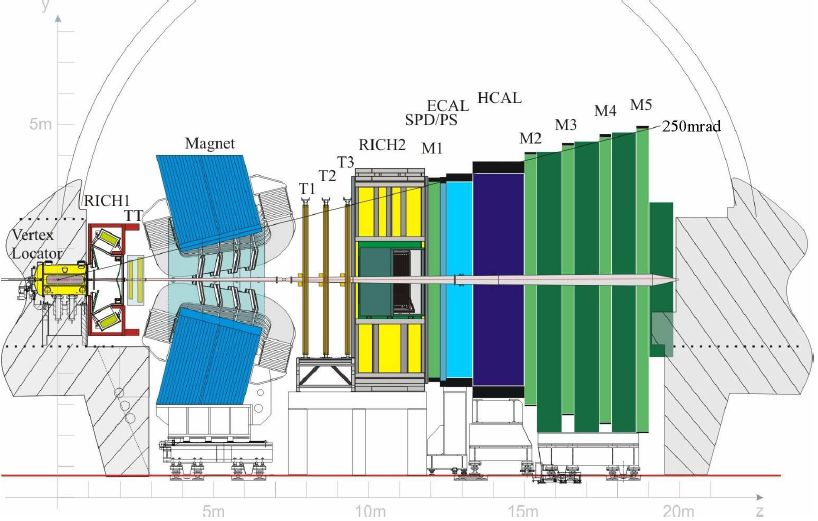
\includegraphics[width=\textwidth]{detektor}
\caption{Schnitt durch die (y,z)-Ebene des LHCb-Detektors. Die Abbildung wurde \cite{detector} entnommen.}
\label{fig:detektor}
\end{figure}


\subsection{Spurdetektoren}
Hauptaufgabe der Spurdektektoren ist die Impulsbestimmung geladener Teilchen. Dazu werden diese durch das Feld eines Dipolmagneten abgelenkt. Die Trajektorien werden mit den Stationen VELO, TT und T1-T3 gemessen, die im Folgenden detaillierter beschrieben werden. Die Ablenkung des Teilchens von seiner ursprünglichen Trajektorie gibt Aufschluss über den Impuls. Das Magnetfeld ist weitestgehend homogen mit einer dominierenden y-Komponente, sodass die Ablenkung hauptsächlich in der (x,z)-Ebene vonstattengeht. Über die Länge $l=10\meter$ integriert beträgt die Feldstärke $\int B\mathrm{d}l = 4\tesla\meter$. Um ladungsabhängige Detektorasymmetrien zu messen, kann die Orientierung des Magnetfeldes umgekehrt werden. \cite{thesis_linn}

\subsubsection{Vertex Locator (VELO)}
Aufgabe des Vertex Locator (VELO) ist die Detektion des Primärvertex (Entstehung eines Teilchens) sowie des Sekundärvertex (erste Interaktion des Teilchens, meist Zerfall). Er ist sehr nah am Kollisionspunkt aus Silikonstreifen aufgebaut und besteht aus 21 Stationen. Um Schäden zu vermeiden, besteht der VELO aus zwei Hälften, die erst zusammengeführt werden, sobald der Teilchenstrahl im Experiment stabil ist.

\subsubsection{Tracker Turicensis (TT)}
Der Tracker Turicensis (TT) besteht aus zwei Stationen, die sich hinter dem Magneten befinden und eine Detektionsfläche von etwa $8,4\meter^2$ bieten. Sie sind wie der VELO aus Silikonstreifen aufgebaut und ermöglichen eine dreidimensionale Spurrekonstruktion, wobei die TT-Stationen so aufgebaut sind, dass die Präzision in der horizontalen Ablenkungsebene (x,z) des Magneten am besten ist. Die Auflösung eines einzelnen Teilchentreffers beträgt etwa $50\micro\meter$.

\subsubsection{Inner Tracker (IT)}
Im Zentrum der drei Stationen T1-T3 nach dem Dipolmagneten ist der sogenannte Inner Tracker platziert. Er ist $120\centi\meter$ breit und $40\centi\meter$ hoch, ebenfalls ein Silikonstreifendetektor und besteht aus vier Schichten, die ähnlich wie die TT Stationen aufgebaut sind. Er deckt eine Fläche von etwa $4\meter^2$ ab und erzielt ebenfalls eine Trefferauflösung von $50\micro\meter$.

\subsubsection{Outer Tracker (OT)}
Der Outer Tracker bildet den äußeren Teil der Stationen T1-T3, der nicht vom IT abgedeckt wird. Er besteht ebenfalls aus 4 Schichten und ist aus Driftröhrchen aufgebaut, die mit einem Gasgemisch aus Argon (70\%), CO$_2$(28,5\%) und O$_2$ (1,5\%) gefüllt sind. Im Innern der Röhrchen verläuft ein mit Gold beschichteter Anodendraht aus Wolfram. Die räumliche Auflösung eines einzelnen Röhrchens liegt bei $200\micro\meter$.

\subsubsection{Klassifizierung von Spuren} \label{kap:spurklassen}
Je nachdem, welche Detektoren getroffen wurden, teilt man die Spuren in vier unterschiedliche Kategorien ein:
\begin{itemize}
\item \textbf{VELO Spuren} enthalten Treffer ausschließlich im VELO und dienen hauptsächlich der Rekonstruktion des Primärvertex.
\item Hinterlassen die Teilchen Treffer im VELO und in den TT-Stationen, spricht man von \textbf{Upstream Spuren}. Hierbei handelt es sich dann um Teilchen mit kleinem Impuls, da der Magnet die Teilchen so stark ablenkt, dass jene den Akzeptanzbereich des Detektors verlassen und die anschließenden Detektoren nicht mehr passieren.
\item Bei \textbf{Downstream Spuren} gibt es nur Treffer in den Stationen TT und T1-T3. Diese treten vor allem bei langlebigen Teilchen wie dem $\Kshort$ auf, die den VELO vor ihrem Zerfall verlassen. In dieser Arbeit werden ausschließlich Downstream Spuren verwendet (siehe dazu auch Kapitel \ref{kap:downstream})
\item Gibt es Treffer in allen Stationen (VELO, TT, T1-T3), so spricht man von \textbf{Long Spuren}. Da es hier die meisten Treffer gibt, haben diese Spuren die präziseste Impulsauflösung. \cite{thesis_linn}
\end{itemize}

\subsection{Detektoren zur Teilchenidentifikation}
Neben der Rekonstruktion der Spuren ist es natürlich essentiell, auch die Teilchen zu identifizieren. Hierzu werden die Informationen der Detektoren RICH1/2, SPD, PS HCAL, ECAL sowie M1-M5 für eine Teilchenhypothese verwendet.

\subsubsection{Die Ring Imaging Cherenkov Detektoren (RICH)}
Die beiden RICH Detektoren nutzen die Cherenkov-Strahlung, um Teilchen voneinander zu unterscheiden, insbesondere $\pi^{\pm}$ und $K^{\pm}$. Ähnlich dem Machschen Kegel bei Schall emittieren geladene Teilchen Photonen in Kegelform, wenn sie ein Medium mit einer Geschwindigkeit $v$ passieren, die größer ist als die Lichtgeschwindigkeit $c'=c/n$ in diesem Medium ($n:$ Brechungsindex des Mediums). Für den Öffnungswinkel $\theta_{\text{C}}$ des Lichtkegels gilt dann:
\begin{align}
\cos \theta_{\text{C}} = \frac{c}{vn}.
\end{align}
Durch Messung des Öffnungswinkels und der Impulsinformation aus den Spurdetektoren lässt sich die Teilchenmasse bestimmen und somit eine Teilchenhypothese aufstellen. RICH1 ist dabei für kleine Impulse im Bereich von $1\giga\electronvolt$ bis $60\giga\electronvolt$ zuständig und deckt den kompletten Akzeptanzbereich des Detektors ab, RICH2 arbeitet dagegen bei Impulsen von $15\giga\electronvolt$ bis $100\giga\electronvolt$ und deckt einen Winkelbereich von ca. $15\milli\rad$ bis $120\milli\rad$ in horizontaler und $100\milli\rad$ in vertikaler Ebene ab.

\subsubsection{Kalorimetersystem}
Das Kalorimetersystem dient zur Identifikation von Elektronen, Photonen sowie Hadronen und soll deren Energie und Position bestimmen. Durch Wechselwirkung mit dem Kalorimetermaterial erzeugen jene einen kaskadenartigen Zerfall. Bei den Subdetektoren des Systems handelt es sich um Szintillationsdetektoren. Diese sind im Einzelnen:
\begin{itemize}
\item Der \textbf{Scintillating Pad Detector (SPD)} kann nur geladene Teilchen detektieren und dient damit der Unterscheidung von Photon und Elektron.
\item Auf den SPD und eine $12\milli\meter$ dicke Bleiplatte folgt der \textbf{Preshower Detector (PS)}. Die Platte löst Kaskaden von Photonen und Elektronen aus. Hadronische Kaskaden beginnen erst später und können damit unterschieden werden.
\item Das \textbf{elektromagnetische Kalorimeter (ECAL)} besteht im Wechsel aus Blei- und Szintillationsplatten und detektiert Photonen- und Elektronenschauer.
\item Beim \textbf{hadronischen Kalorimeter (HCAL)} wechseln sich Eisen- und Szintillationsplatten ab. Er ist sensitiv für hadronische Kaskaden.
\end{itemize}

\subsubsection{Myonkammern}
Der LHCb-Detektor besitzt insgesamt 5 Myonenkammern (M1-M5). Zur Verbesserung der Impulsmessung im Trigger ist M1 vor den Kalorimetern angebracht, die restlichen am Ende des Detektors. Zwischen M2-M5 befinden sich $80\centi\meter$ dicke Eisenplatten zur Absorption hadronischer Teilchen. Ab einem Impuls von etwa $6\giga\electronvolt/c$ können die Myonen alle 5 Stationen passieren. \cite{thesis_linn}

\subsection{Trigger}
Der LHCb-Detektor besitzt ein dreistufiges Triggersystem, um die Ereignisrate von $40\mega\hertz$ auf $2-3\kilo\hertz$ zu reduzieren. Die hierin enthaltenen Informationen werden dann zur weiteren Bearbeitung gespeichert. Die drei Stufen bestehen aus dem Hardwaretrigger \textbf{L0}, der die Ereignisrate auf $1\mega\hertz$ senkt, sowie den beiden software-basierten \glqq High Level Trigger\grqq\ \textbf{HLT1}($50\kilo\hertz$) und \textbf{HLT2}($2-3\kilo\hertz$). Für die Trigger siehe auch Kapitel \ref{kap:trigger}.
\chapter{CP-Verletzung in B-Meson-Systemen}

\section{B-Mesonen und der Zerfallskanal \Decaychannel}
\subsection{Das Standardmodell der Teilchenphysik}
Im Standardmodell der Teilchenphysik gibt es 17 elementare Bausteine der Materie (siehe Abb. \ref{fig:standardmodell}): 12 Fermionen, davon 6 Quarks (u, d, c, s, t, b), die sich im engeren Sinne zur Materie hadronisieren oder Mesonen bilden, und 6 Leptonen (e, $\mathrm{\mu}$, $\mathrm{\tau}$ sowie die jweiligen Neutrinos $\mathrm{\nu_e}$, $\mathrm{\nu_{\mu}}$, $\mathrm{\nu_{\tau}}$). Von diesen 12 Fermionen existieren jeweils noch Antiteilchen (gleiche Eigenschaften, aber entgegengesetzte Masse). Das Standardmodell enthält weiterhin 4 Eichbosonen (Photon, Gluon, Z- und W$^{\pm}$-Boson), die die 3 der 4 elementaren Kräfte übertragen: die elektromagnetische, starke und schwache Wechselwirkung. Das für die Gravitation postulierte Graviton konnte bislang nicht nachgewiesen werden. Ergänzt wird das Standardmodell, durch das Higgs-Boson, welches als Teil des Higgs-Mechanismus den Elementarteilchen seine Masse verleiht und Gegenstand aktueller Forschung ist. Mit hoher Wahrscheinlichkeit gelang jüngst der Nachweis des Higgs am CERN \cite{higgs}.

\begin{figure}[hptb]
\centering
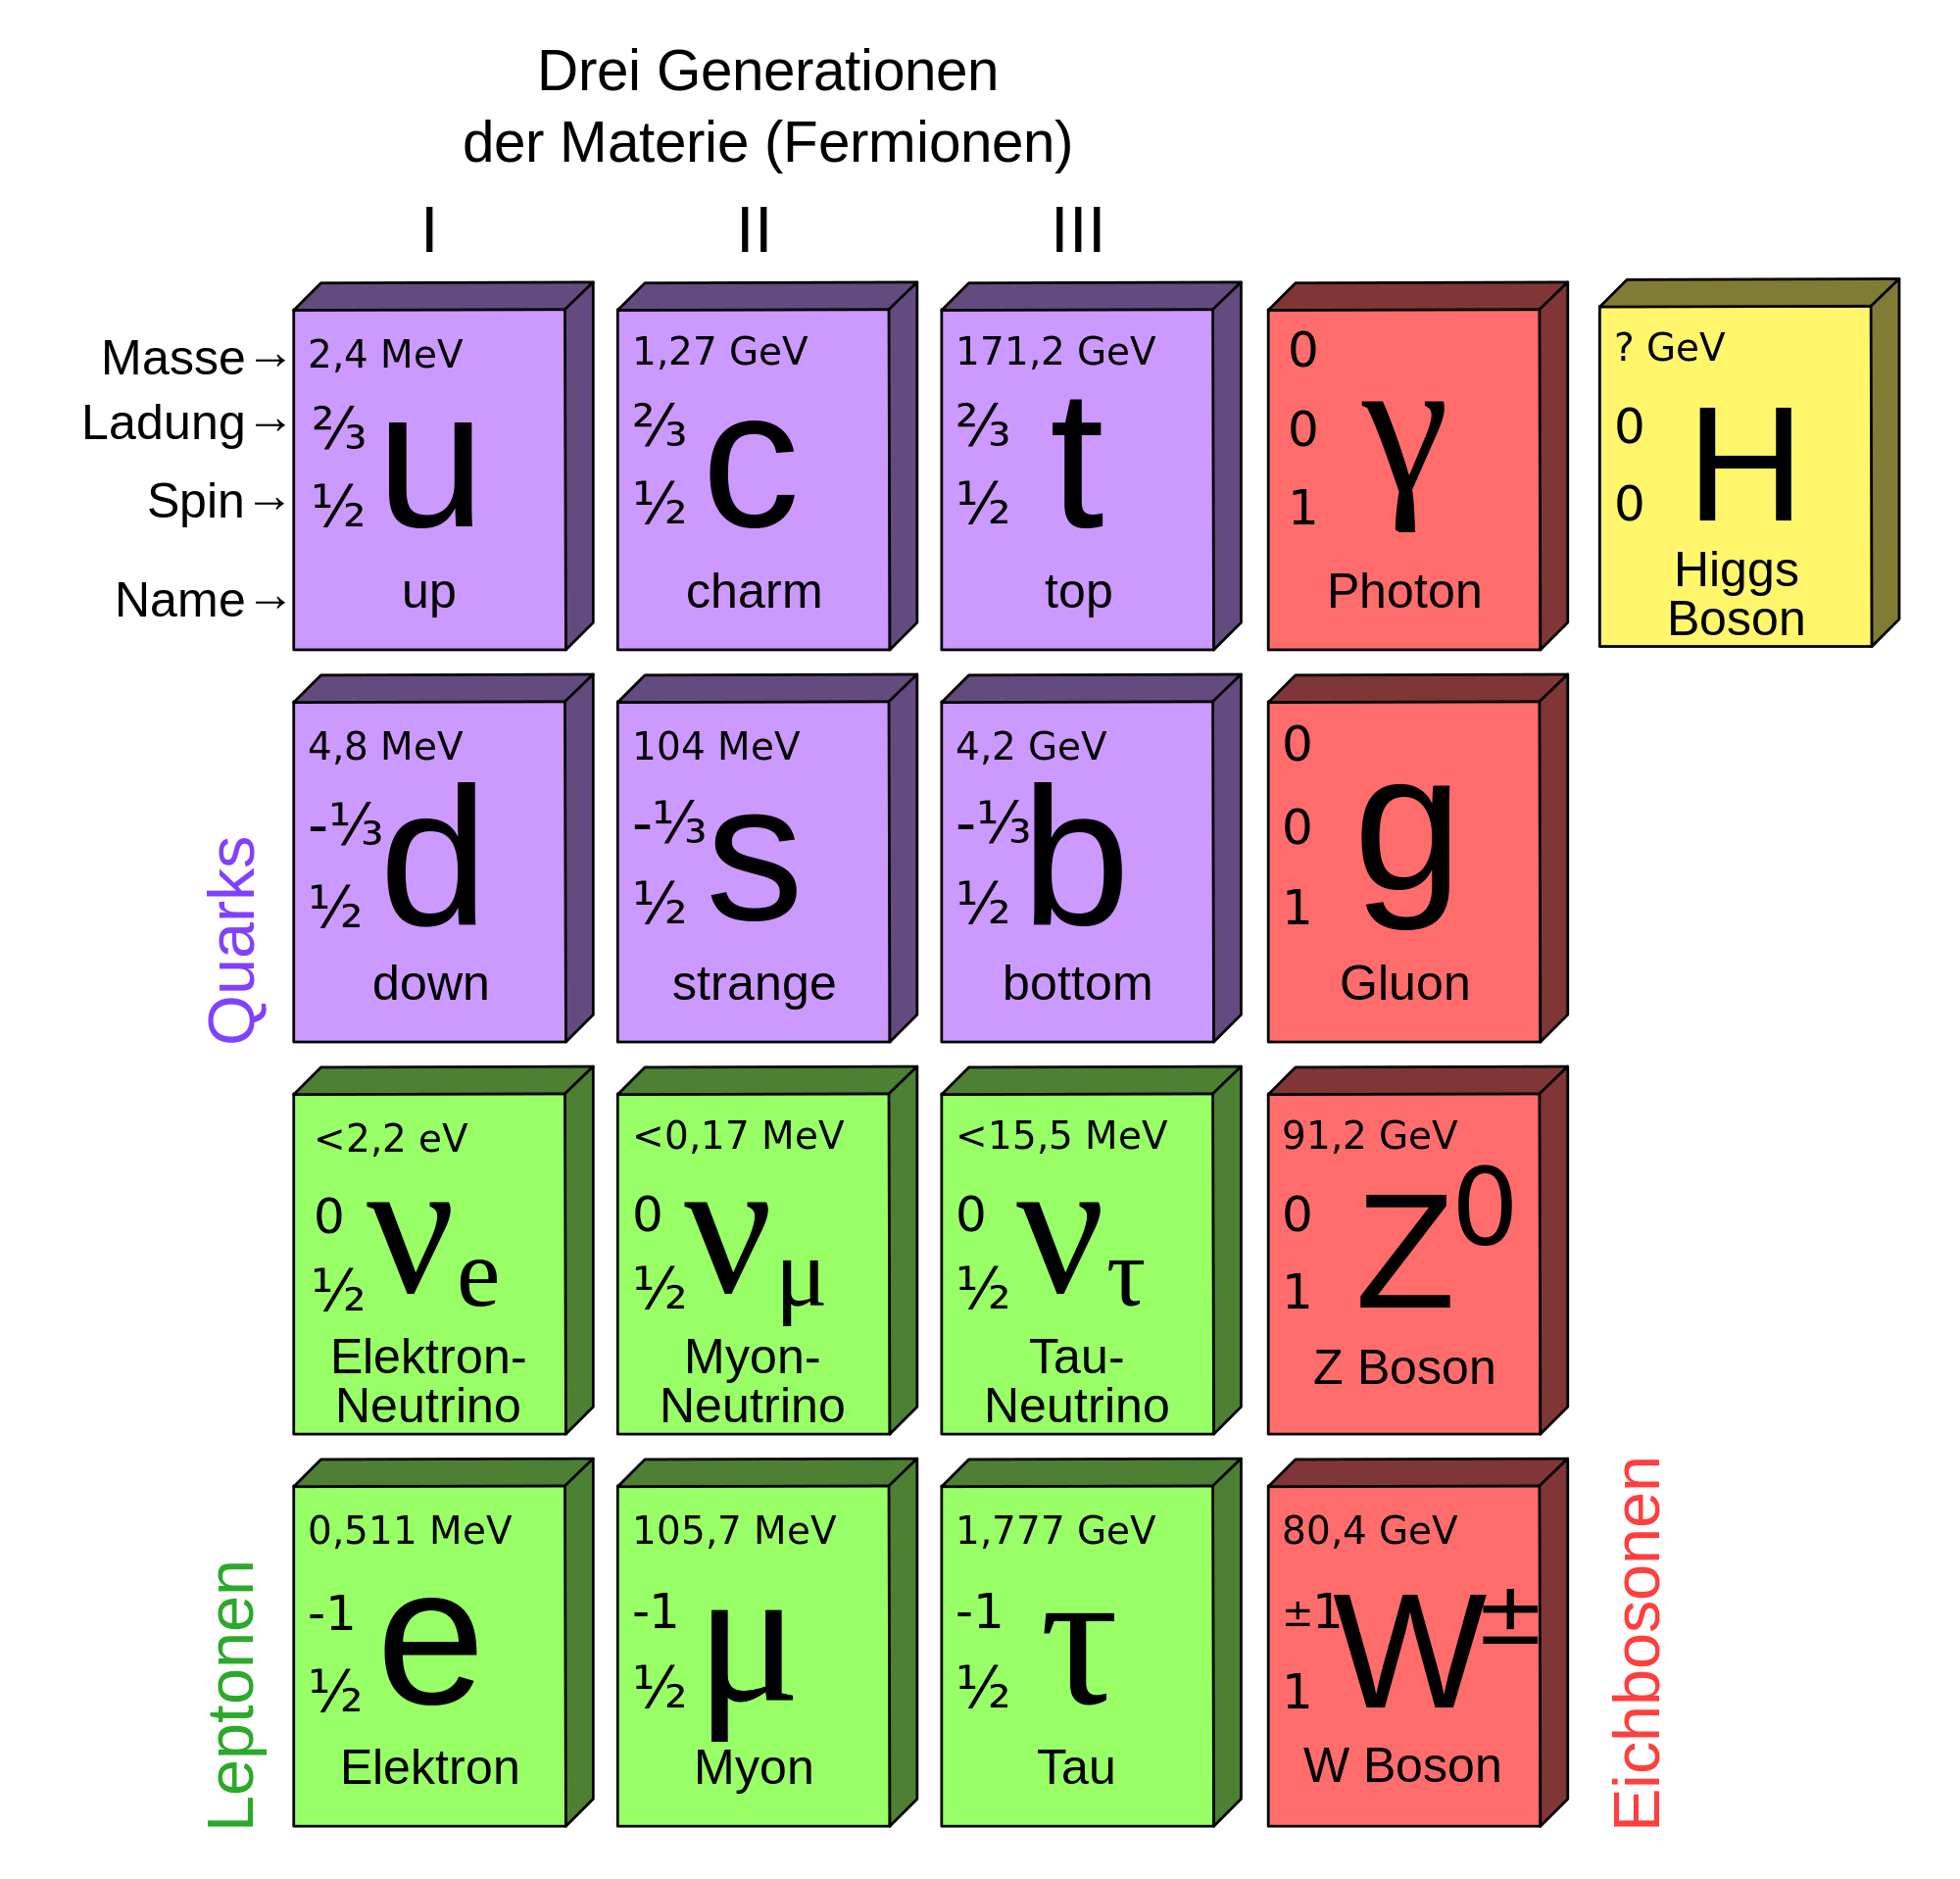
\includegraphics[width=0.5\textwidth]{standardmodell}
\caption{Das Standardmodell der Teilchenphysik \cite{wiki_standard}}
\label{fig:standardmodell}
\end{figure}

\subsection{B-Mesonen und ihre Mischung}
Mesonen sind Paare aus Quarks und Antiquarks beliebigen Flavours. B-Mesonen insbesondere bestehen aus einem Anti-b-Quark ($\mathrm{\overline{b}}$) mit einem u-, d-, c- oder s-Quark beziehungsweise aus der Kombination der jeweiligen Antiteilchen (Anti-B-Mesonen).

Die in dieser Arbeit betrachteten \Bd-Mesonen haben demnach die Quarkzusammensetzung $\Ket{\text{\Bd}} = \Ket{\overline{b}d}$ und sind elektrisch neutral. Solch neutrale Mesonen besitzen die Eigenschaft, dass sie sich in ihre Antiteilchen wandeln können und umgekehrt. Es findet folglich eine Oszillation zwischen \Bd und \Bdbar statt, die man auch Mischung nennt. Abbildung \ref{fig:bmixing} zeigt zwei mögliche Feynmangraphen für diesen Prozess. Innerhalb der Schleifen kann die Energieerhaltung kurzzeitig verletzt werden, sodass auch kurzerhand die deutlich schweren top-Quarks enstehen können. Zu diesem Mischungsprozess leisten sie sogar einen dominanten Beitrag. Präzise Messungen der \Bd-Mischung erlauben Aussagen bspw. über die top-Masse und grenzen damit das Standardmodell ein, gleichzeitig erhofft man sich, durch noch präzisere Messungen Hinweise auf \glqq neue Physik\grqq zu finden, die sich dann in kleinsten Korrekturen innerhalb der Schleife bemerkbar machen würden.

\begin{figure}[hptb]
\centering
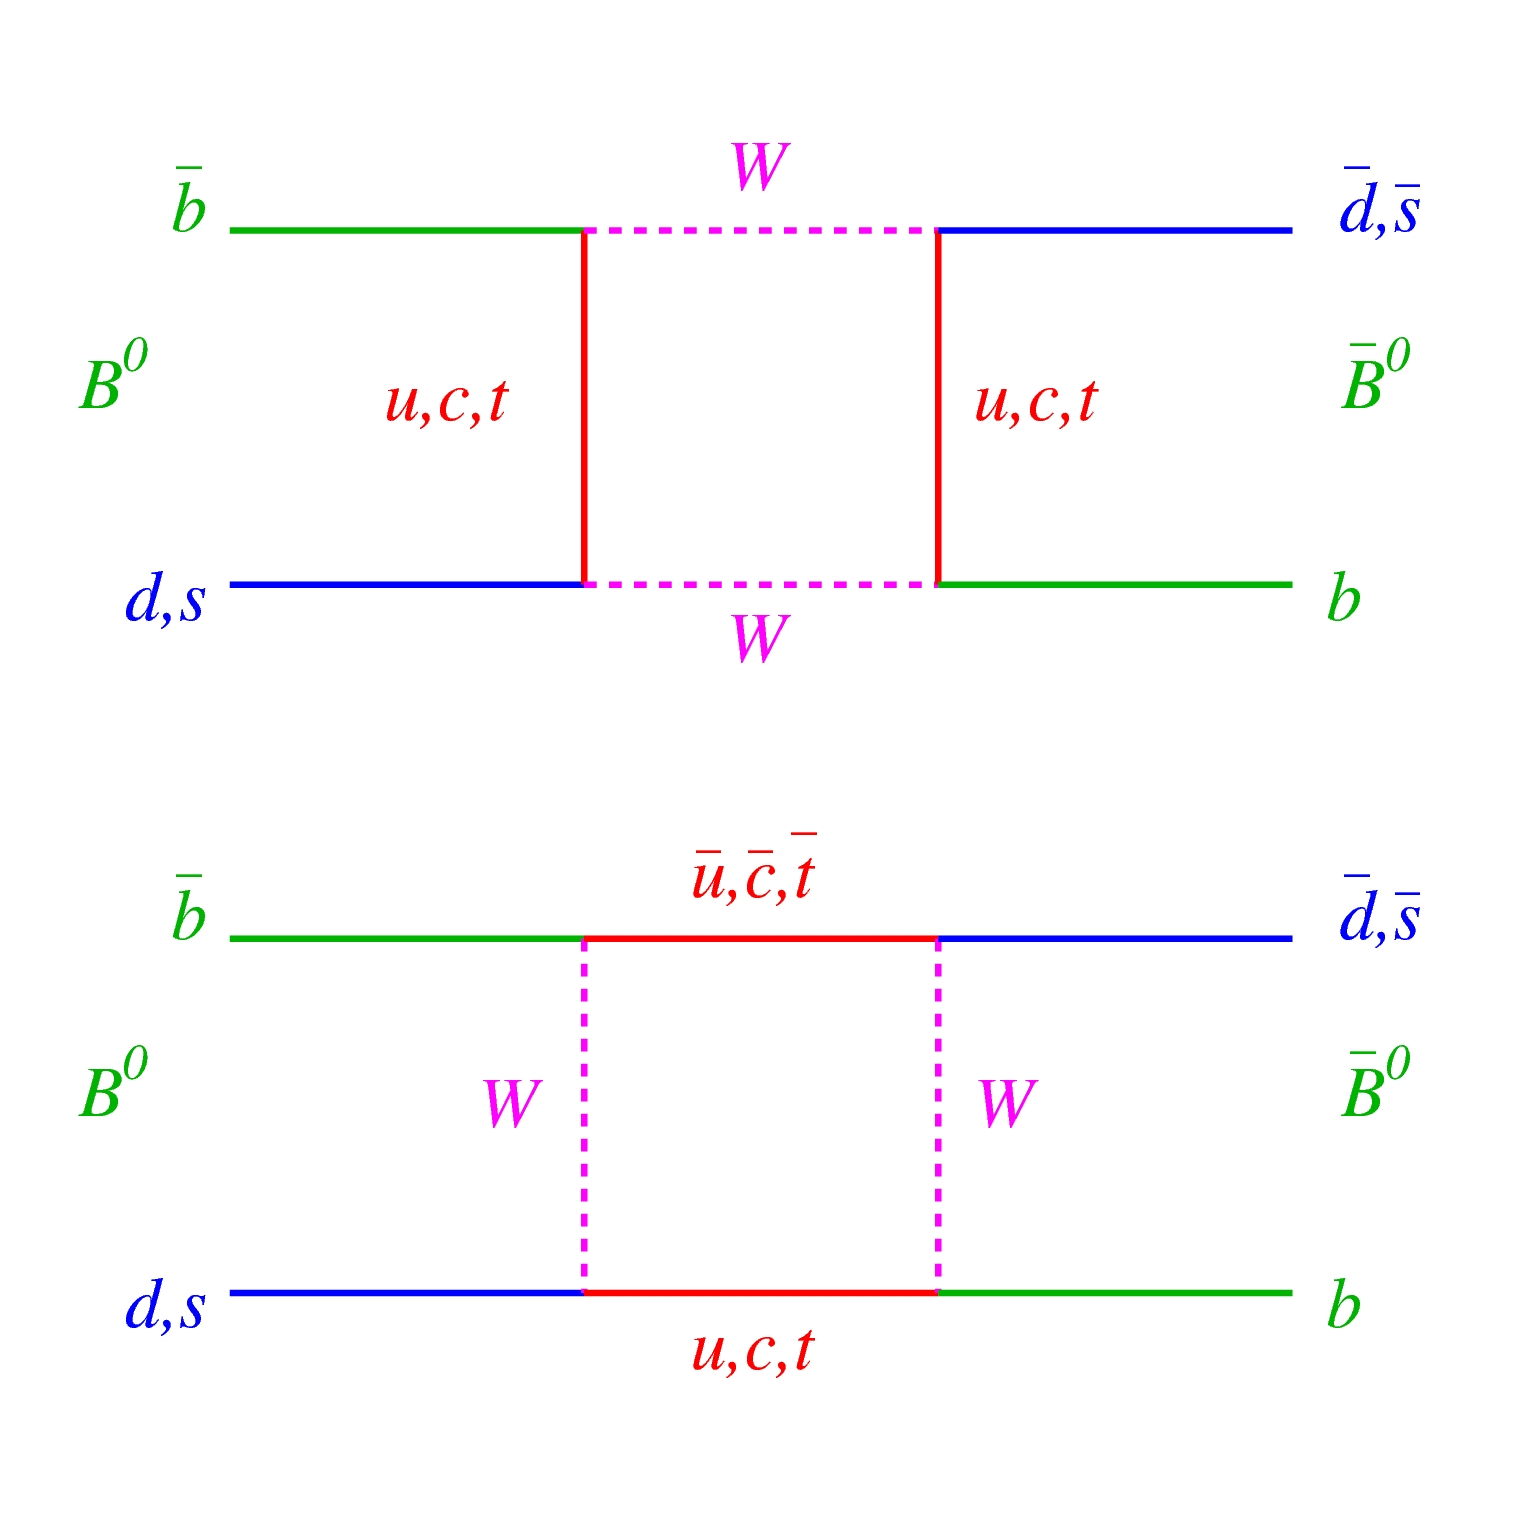
\includegraphics[width=0.5\textwidth]{bmixing}
\caption{Feynmangraphen zur Mischung von \Bd- und \Bdbar-Mesonen}
\label{fig:bmixing}
\end{figure}


\subsection{Der Zerfallskanal \Decaychannel}
In dieser Arbeit wird der Zerfallskanal \Decaychannel betrachtet. Abbildung \ref{fig:decay} zeigt entsprechende Feynmangraphen. Jener Kanal ist auch als \glqq goldener\grqq Zerfallskanal für die Messung der \CP-Verletzung bekannt. Hintergrund ist, dass der Endzustand $\Ket{\JPsi\Kshort}$ ein \CP-Eigenzustand ist ($\text{\CP}\Ket{\JPsi\Kshort} = - \Ket{\JPsi\Kshort}$). Die Teilchen $\JPsi$ und $\Kshort$ haben die Flavoureigenzustände $\Ket{\JPsi} = \Ket{c\overline{c}}$ sowie $\Ket{\Kshort} = \tfrac{1}{\sqrt{2}}\left(\Ket{d\overline{s}}-\Ket{s\overline{d}}\right)$. Diese Teilchen sind ebenfalls nicht stabil und zerfallen unter anderem weiter gemäß $\JPsi \rightarrow \mu^+\mu^-$ und $\Kshort \rightarrow \pi^+\pi^-$, was zur Rekonstruktion der \Bd-Mesonen im Detektor genutzt wird.

\begin{figure}[hptb]
\centering
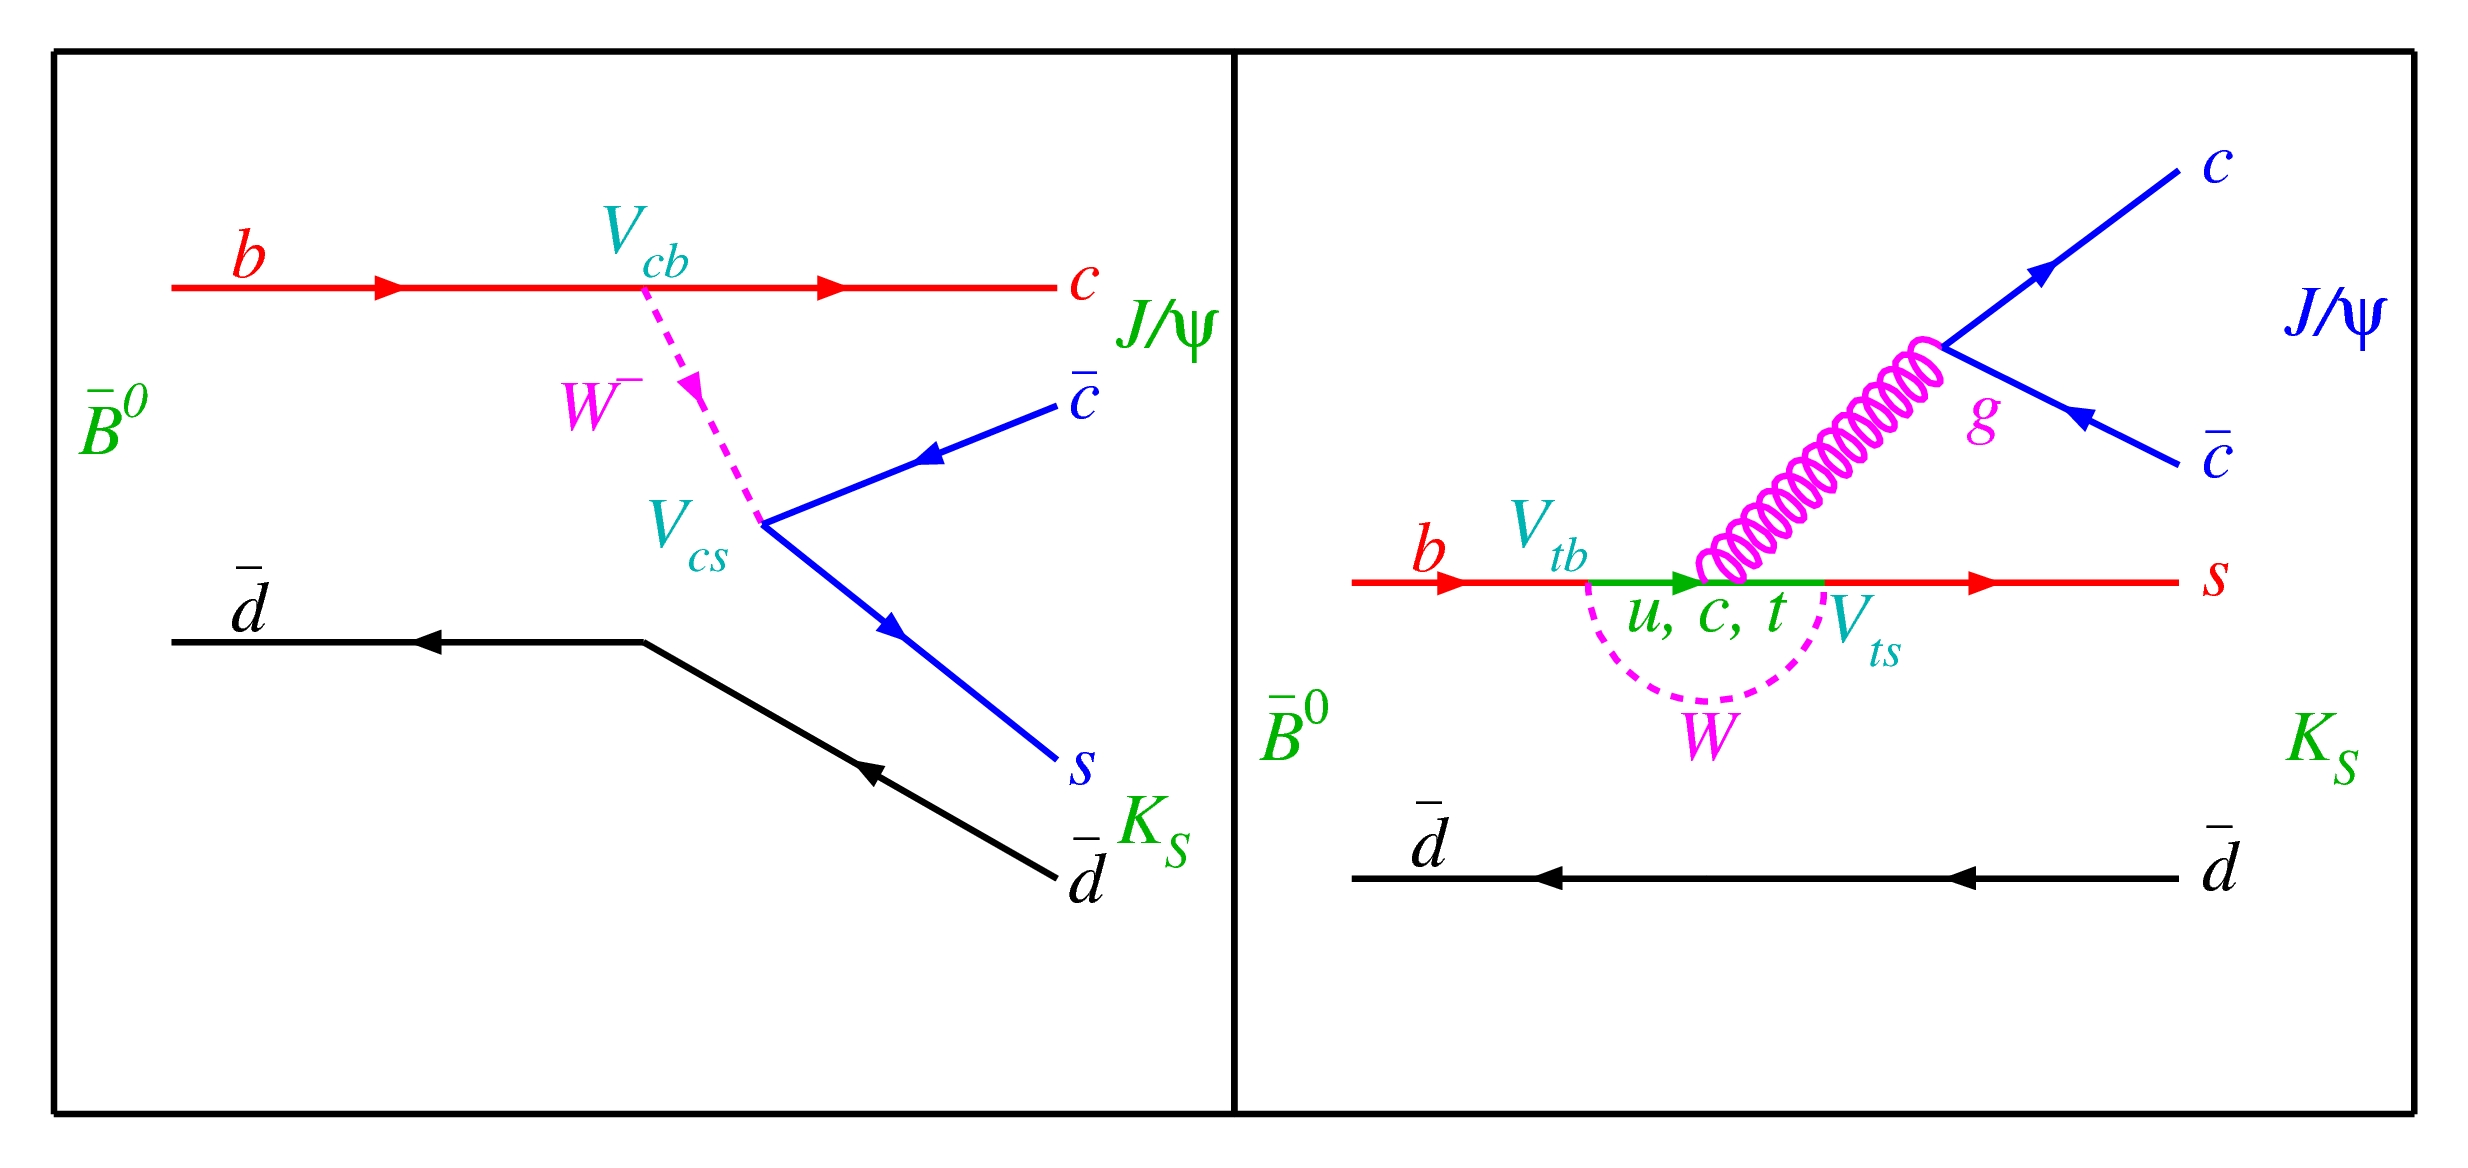
\includegraphics[width=\textwidth]{bd2jpsikshort}
\caption{Feynmangraph zum Zerfall \Decaychannel. Links: Baumdiagramm, rechts: Pinguindiagramm}
\label{fig:decay}
\end{figure}

\section{Diskrete Symmetrietransformationen}
Symmetrien sind in der Physik von zentraler Bedeutung. Gemäß dem Noether-Theorem existiert in der klassischen Physik zu jeder kontinuierlichen Symmetrie eine Erhaltungsgröße. In quantenmechanischen Systemen können wir drei diskrete Symmetrietransformationen betrachten:
\begin{enumerate}
\item \textbf{Parität $\mathcal{P}$:} \\
      Bei der Paritätsoperation wird das Vorzeichen der kartesischen Ortskoordinaten umgekehrt. Dies entspricht einer Punktspigelung.
\item \textbf{Ladungskonjugation $\mathcal{C}$:} \\
      Jedes Teilchen wird durch sein Antiteilchen ersetzt.
\item \textbf{Zeitumkehr $\mathcal{T}$:} \\
      Das Vorzeichen auf der Zeitachse wird umgekehrt. Da in der vorligenden Arbeit allerdings nur die CP-Verletzung gemessen werden soll, wird die Zeitumkehr im folgenden vernachlässigt.
\end{enumerate}
Entgegen der klassischen Intuition konnte Wu 1956 nachweisen, dass die Parität im $\beta$-Zerfall und damit in der schwachen Wechselwirkung nicht erhalten ist. Weitere Experimente zeigen, dass die schwache Wechselwirkung die Parität maximal verletzt: Neutrinos, die nur schwach wechselwirken können, sind stets \glqq linkshändig\grqq (Spin und Impuls antiparallel), Antineutrinos dagegen immer \glqq rechtshändig\grqq (Spin und Impuls parallel). Da der Spin im Gegensatz zum Impuls invariant unter $\mathcal{P}$-Transformation ist, würde diese Operation aus einem linkshändigen Neutrino ein rechtshändiges machen, was in der Nautr nicht realisiert ist.

Damit ist offensichtlich, dass die schwache Wechselwirkung auch die Ladungskonjugation verletzt: Wendet man die $\mathcal{C}$-Transformation auf ein linkshändiges Neutrino an, so erhält man ein linkshändiges Antineutrino. Dieses existiert aber wie bereits erwähnt nicht. Analog gilt die Überlegung auch für Antineutrinos.

\subsection{Scheinbare $\mathcal{CP}$-Invarianz}
Wendet man nun aber die Transformationen $\mathcal{P}$ und $\mathcal{C}$ direkt hintereinander an, so ergibt sich zunächst kein Widerspruch zur Natur (siehe Abb. \ref{fig:cp_invarianz}). Aus einen linkshändigen Neutrino wird ein rechtshändiges Antineutrino. Im Jahre 1964 wurde dann allerdings im Zerfall neutraler K-Mesonen erstmals $\mathcal{CP}$-Verletzung nachgewiesen. \cite{kleinknecht}

\begin{figure}[hptb]
\centering
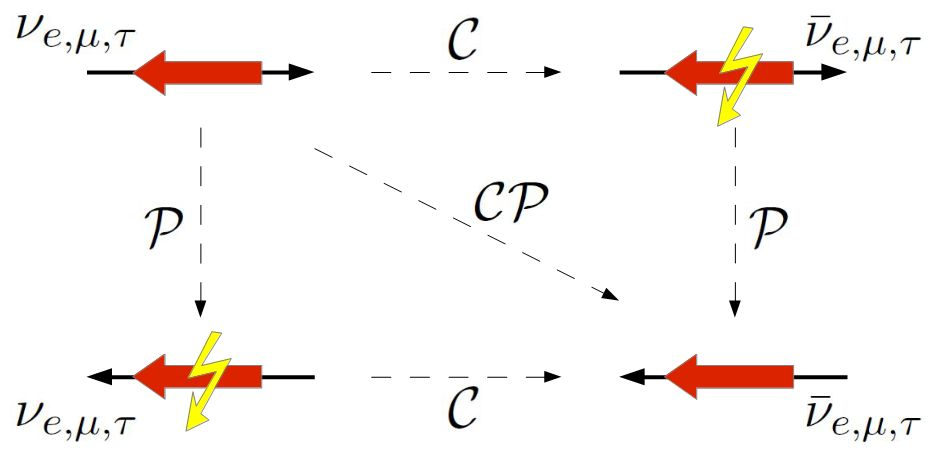
\includegraphics[width = 0.8\textwidth]{cp_invarianz}
\caption{Scheinbare $\mathcal{CP}$-Invarianz: Während eine reine $\mathcal{P}$- oder $\mathcal{C}$-Transformation zu in der Natur nicht realisierten Zuständen führt, scheint es bei der kombinierten $\mathcal{CP}$-Transformation keinen Widerspruch zu geben (dünne Pfeile: Impulsausrichtung, dicke Pfeile: Spinausrichtung).}
\label{fig:cp_invarianz}
\end{figure}



\section{\CP-Verletzung in der Mischung}
Die Flavoureigenzustände $\Ket{B^0} = \Ket{\overline{b}d}$ und $\Ket{\overline{B^0}} = \Ket{b\overline{d}}$ entsprechen nicht den Masseneigenzuständen. Wir definieren daher die normierten Zustände
\begin{align}
\Ket{B_h} = p \Ket{B^0} - q \Ket{\overline{B^0}} \label{eq:b_heavy}\\ 
\Ket{B_l} = p \Ket{B^0} + q \Ket{\overline{B^0}} \label{eq:b_light}\\
\text{mit} \quad |p|^2 + |q|^2 = 1
\end{align}
welche eine definierte Masse und Zerfallsbreite besitzen. Sie sind auch Eigenzustände eines nicht-hermiteschen Hamiltonoperators (Nichthermitizität wegen des möglichen Zerfalls der Teilchens). Dieser setzt sich zusammen aus den hermiteschen Massenoperatoren $M$ und $\Gamma$. Notieren wir die lineare Superposition der Zustände \ref{eq:b_heavy} und \ref{eq:b_light} als $\begin{pmatrix} p \\ q \end{pmatrix}$, so nimmt die zeitabhängige Schrödingergleichung die Form
\begin{align}
\im \diff{}{t}\begin{pmatrix} p \\ q \end{pmatrix} = \left(M - \frac{\im}{2} \Gamma\right) \begin{pmatrix} p \\ q \end{pmatrix}
\end{align}
an und führt zur folgenden zeitlichen Entwicklung der Zustände:
\begin{align}
\nonumber \Ket{B_{h/l}(t)} &= \e^{-\im m_{h/l}t-\frac{1}{2}\Gamma_{h/l}t}\Ket{B_{h/l}(0)} \\
                           &= \e^{-\gamma_{h/l}t}(p\Ket{B^0} \mp q\Ket{\overline{B^0}}) \\
&\text{mit} \quad \gamma_{h/l} = \im m_{h/l}+\frac{\Gamma_{h/l}}{2}
\end{align}
Hierbei ist $\gamma_{h/l}$ so definiert, dass $-\im\gamma_{h/l} = m_{h/l}-\frac{\im}{2}\Gamma_{h/l}$ die Eigenwerte des Hamiltonoperators $\mathcal{H} := \left(M - \frac{\im}{2} \Gamma\right)$ sind. Umgeschrieben auf die Flavoureigenzustände erhält man:
\begin{align}
\nonumber \Ket{B^0(t)} &= \frac{1}{2p}\left(\Ket{B_h} + \Ket{B_l}\right) \\
                       &= \frac{1}{2}\left[ (\e^{-\gamma_h t}+\e^{-\gamma_l t})\Ket{B^0} - \frac{q}{p}(\e^{-\gamma_h t}-\e^{-\gamma_l t})\Ket{\overline{B^0}}\right] \label{eg:b(t)}
\end{align}
Die Wahrscheinlichkeit für den Übergang eines $\Ket{B^0}$ (zum Zeitpunkt $t=0$) in ein $\Ket{\overline{B^0}}$ beträgt:
\begin{align}
\nonumber P(B^0\rightarrow\overline{B^0})(t) &= |\Braket{\overline{B^0}|B^0(t)}|^2 \\
                                        &= \frac{1}{4} \left|\frac{q}{p}\right|^2 \left[\e^{-\Gamma_h t} + \e^{-\Gamma_l t} - 2\e^{-\frac{1}{2}(\Gamma_h + \Gamma_l) t}\cos(\Delta m_d t)\right] \\
&\text{mit} \quad \Delta m_d = m_h - m_l
\end{align}

Analog gilt für die Übergangswahrscheinlichkeit eines $\Ket{\overline{B^0}}$ in ein $\Ket{B^0}$:
\begin{align}
P(\overline{B^0}\rightarrow B^0)(t) = \frac{1}{4} \left|\frac{p}{q}\right|^2 \left[\e^{-\Gamma_h t} + \e^{-\Gamma_l t} - 2\e^{-\frac{1}{2}(\Gamma_h + \Gamma_l) t}\cos(\Delta m_d t)\right] 
\end{align}

Es kommt daher in der Mischung zur \CP-Verletzung, wenn die Oszillation ungleichmäßig verläuft, anders ausgedrückt:
\begin{align}
\text{\CP-Verletzung in der Mischung} \qquad \Longleftrightarrow \qquad \left|\frac{p}{q}\right| \neq 1 
\end{align}

\section{Direkte \CP-Verletzung}
Die Zerfallsamplituden der neutralen $B^0$-Mesonen in einen Endzustand $\Ket{f}$ bzw. seinen \CP-konjugierten Zustand $\Ket{\overline{f}}$ sind definiert als
\begin{alignat}{2}
\nonumber A_f &= \Braket{f|\mathcal{H}|B^0}, && \qquad A_{\overline{f}} = \Braket{\overline{f}|\mathcal{H}|B^0}, \\
          \overline{A_f} &= \Braket{f|\mathcal{H}|\overline{B^0}}, && \qquad  \overline{A_{\overline{f}}} = \Braket{\overline{f}|\mathcal{H}|\overline{B^0}}. \label{eq:decay_amplitudes}
\end{alignat}
Dabei bezeichnet $\mathcal{H}$ einen Hamiltonoperator der schwachen Wechselwirkung. Ist \CP erhalten, dann sollten die Zerfallsraten, ergo auch die Zerfallsamplituden eines $B^0$ nach $f$ sowie eines $\overline{B^0}$ nach $\overline{f}$ gleich sein. Dies bedeutet:
\begin{align}
\text{Direkte \CP-Verletzung} \qquad \Longleftrightarrow \qquad \frac{|A_f|}{|\overline{A_{\overline{f}}}|} \neq 1 \quad \text{bzw.} \quad \frac{|\overline{A_f}|}{|A_{\overline{f}}|} \neq 1
\end{align}


\section{\CP-Verletzung in der Interferenz}
Die Zustände \ref{eq:b_heavy} und \ref{eq:b_light} haben eine nahezu gleiche Anzahl an Zerfällskanäle. Dies hat zur Folge, dass die Lebensdauern des schweren und leichten Zustands innerhalb weniger Prozent gleich sind:
\begin{align}
\Gamma := \Gamma_h = \Gamma_l \label{eq:Gamma}
\end{align}

Weiterhin sagt das Standard Modell nur eine kleine \CP-Verletzung in der \Bd - \Bdbar - Mischung voraus, sodass
\begin{align}
\left|\frac{p}{q}\right| = 1 \qquad \text{in} \mathcal{O}(10^{-3}). \label{eg:pq_approx}
\end{align}

Für das B-Meson-System bleibt daher nur die Möglichkeit der \CP-Verletzung in der Interferenz von Mischung und direktem Zerfall. Der in dieser Arbeit betrachtete Zerfallskanal $B_d^0 \rightarrow J/\Psi K_s^0$ hat einen \CP-Eigenzustand als Endzustand (\CP $\Ket{\JPsi\Kshort} = -\Ket{\JPsi\Kshort}$). In Anlehnung an \ref{eq:decay_amplitudes} sind die Zerfallsamplituden hier definiert als
\begin{align}
\nonumber A_f := \Braket{f|B^0(t)}, \qquad \overline{A_{f}} := \Braket{f|\mathcal{H}|\overline{B^0}}
\end{align}

Mit Blick auf die Zerfallsamplituden der Masseneigenzustände wird die komplexe Größe
\begin{align}
\lambda_f := \frac{q\overline{A_f}}{pA_f} \label{eq:lambda}
\end{align}
definiert. Ausgehend von Gleichung \ref{eg:b(t)} sowie mit Hilfe fer Gleichungen (\ref{eq:Gamma}), (\ref{eg:pq_approx}) und (\ref{eq:lambda}) gilt für die Zerfallsrate eines anfänglich reinen \Bd-Zustands:
\begin{align}
\nonumber \Gamma (B^0 \rightarrow \JPsi\Kshort) &= \frac{1}{4}\left| (\e^{-\gamma_h t}+\e^{-\gamma_l t})A_f - \frac{q}{p}(\e^{-\gamma_h t}-\e^{-\gamma_l t})\overline{A_f}\right|^2 \\
&= \frac{1}{2} \left|A_f\right|^2\e^{-\Gamma t} \left[1+|\lambda_f|^2 + (1-|\lambda_f|^2)\cos(\Delta m_d t) - 2\mathrm{Im}(\lambda_f)\sin(\Delta m_d t)\right]
\end{align}
Analog:
\begin{align}
\Gamma (\overline{B^0} \rightarrow \JPsi\Kshort) &= \frac{1}{2} \left|A_f\right|^2\e^{-\Gamma t} \left[1+|\lambda_f|^2 -(1-|\lambda_f|^2)\cos(\Delta m_d t) + 2\mathrm{Im}(\lambda_f)\sin(\Delta m_d t)\right]
\end{align}

Damit kann die vom Standard Modell prognostizierte \CP-verletzende Asymmetrie 
\begin{align}
\mathcal{A}_{\text{\CP}} &= \frac{\Gamma (\overline{B^0} \rightarrow \JPsi\Kshort) - \Gamma (B^0 \rightarrow \JPsi\Kshort)}{\Gamma (\overline{B^0} \rightarrow \JPsi\Kshort) + \Gamma (B^0 \rightarrow \JPsi\Kshort)} \\
&= -\frac{1-|\lambda_f|^2}{1+|\lambda_f|^2}\cos(\Delta m_d t) + \frac{2\mathrm{Im}(\lambda_f)}{1+|\lambda_f|^2}\sin(\Delta m_d t) \\
&=: \CJPsi \cos(\Delta m_d t) + \SJPsi \sin(\Delta m_d t)
\end{align}
berechnet werden und vereinfacht sich - da $\Ket{\JPsi\Kshort}$ ein \CP-Eigenzustand ist, gilt $|\lambda_f| = 1$ - hier zu
\begin{align}
\mathcal{A}_{\text{\CP}} = \mathrm{Im}(\lambda_f)\sin(\Delta m_d t) .
\end{align}

Damit kann im B-Meson-System, insbesondere im Zerfall $B_d^0 \rightarrow J/\Psi K_s^0$ durch Messung der Asymmetrie-Amplitude $\SJPsi$ \CP-Verletzung in der Interferenz gemessen werden.

\begin{align}
\text{\CP-Verletzung in der Interferenz} \qquad \Longleftrightarrow \qquad \SJPsi = \mathrm{Im}(\lambda)\neq 0
\end{align}

\section{CKM-Formalismus}
Durch Austausch eines W$^{\pm}$-Bosons können Quarks ihren Flavour ändern. Dabei sind sie aber nicht an ihre jeweilige Generation gebunden, sondern können - wenn auch zum Teil stark unterdrückt - prinzipiell den Flavour einer jeden Generation annehmen. Ein kleines Beispiel: Der Eigenzustand $\Ket{u}$ der starken Wechselwirkung geht über den schwachen Prozess (Austausch eines W$^{\pm}$-Bosons) nicht in ein $\Ket{d}$ über, sondern vielmehr in eine Linearkombination aus $\Ket{d}$, $\Ket{s}$ und $\Ket{b}$, die im folgenden mit $\Ket{d'}$ bezeichnet wird. Allgemein werden die möglichen Linearkombinationen durch die Cabibbo-Kobayashi-Maskawa-Matrix (kurz: CKM-Matrix) beschrieben.
\begin{align}
\begin{pmatrix}
\Ket{d'} \\ \Ket{s'} \\ \Ket{b'}
\end{pmatrix}
=
\begin{pmatrix}
V_{ud} & V_{us} & V_{ub} \\
V_{cd} & V_{cs} & V_{cb} \\
V_{td} & V_{ts} & V_{tb} \\
\end{pmatrix}
\cdot
\begin{pmatrix}
\Ket{d} \\ \Ket{s} \\ \Ket{b}
\end{pmatrix}
\end{align}

Das Betragsquadrat eines jeden Matrixelementes $|V_{ij}|^2$ gibt dabei die Wahrscheinlichkeit für den Übergang eines Quarks $\Ket{i}$ in ein $\Ket{j}$ an. Da die $V_{ij}$ prinzipiell komplex sein können, gibt es zunächst 18 freie Parameter, die zu bestimmen sind. Diese Zahl reduziert sich zum einen um 5 relative Quarkphasen, die physikalisch nicht beobachtbar sind. Zum anderen reduziert die Forderung nach Unitarität der CKM-Matrix die Zahl der unabhängigen Parameter um 9, sodass am Ende 4 Parameter, 3 Euler Winkel sowie eine Phase, welche für die \CP-Verletzung verantwortlich ist, zu bestimmen sind. Die CKM-Matrix lässt sich näherungsweise durch die Wolfenstein-Parametrisierung darstellen:

\begin{align}
V_{\text{CKM}}=
\begin{pmatrix}
V_{ud} & V_{us} & V_{ub} \\
V_{cd} & V_{cs} & V_{cb} \\
V_{td} & V_{ts} & V_{tb} \\
\end{pmatrix}
=
\begin{pmatrix}
1-\frac{\lambda^2}{2} & \lambda & A\lambda^3(\rho-\im\eta) \\
-\lambda & 1-\frac{\lambda^2}{2} & A\lambda^2 \\
A\lambda^3(1-\rho-\im\eta) & -A\lambda^2 & 1
\end{pmatrix}
+ \mathcal{O}(\lambda^4)
\end{align}

Für den Zerfall von \Bd-Mesonen ist die Unitaritätsbedingung
\begin{align}
V_{ud}V_{ub}^* + V_{cd}V_{cb}^* + V_{td}V_{tb}^* = 0
\end{align}
von besonderer Bedeutung. Man kann die einzelnen Summanden nun in der $(\rho,\eta)$-Ebene auftragen und erhält dabei ein sogenanntes Unitaritätsdreieck. Es wird so normiert, dass die Unterseite bei (0,0) beginnt und bei (1,0) endet (siehe Abb. \ref{fig:unitarity}). Die obere Ecke liegt dann bei $(\overline{\rho}, \overline{\eta})$, wobei $\overline{\rho} = \rho(1-\lambda^2/2)$ und $\overline{\eta} = \eta(1-\lambda^2/2)$ gemäß der Wolfenstein-Parametrisierung sind. Die Winkel des Dreiecks erhält man über
\begin{align}
\alpha = \text{arg}\left[-\frac{V_{td}V_{tb}^*}{V_{ud}V_{ub}^*}\right], \qquad
\beta = \text{arg}\left[-\frac{V_{cd}V_{cb}^*}{V_{td}V_{tb}^*}\right], \qquad
\gamma = \text{arg}\left[-\frac{V_{ud}V_{ub}^*}{V_{cd}V_{cb}^*}\right].
\end{align}

\begin{figure}[hptb]
\centering
%\includegraphics[width=\textwidth]{•}
\caption{Unitaritätsdreieck}
\label{fig:unitarity}
\end{figure}

Das Standardmodell stellt für den hier untersuchten Zerfallskanal eine Beziehung zwischen dem Winkel $\beta$ und der komplexen Größe $lambda_f$ aus Gleichung \ref{eq:lambda} her (\cite{nir}, \cite{noguchi}):
\begin{align}
&\lambda_f = \underbrace{\frac{V_{td}V_{tb}^*}{V_{td}^*V_{tb}}}_{\frac{q}{p}} \underbrace{\frac{V_{cd}^*V_{cb}}{V_{cd}V_{cb}^*}}_{\frac{\overline{A_f}}{A_f}} = \e^{2\im\beta} \\
\Longrightarrow &\SJPsi = \mathrm{Im}(\lambda_f) = \sin(2\beta).
\end{align}
 
Durch Messung der Amplitude der \CP-Asymmetrie kann man direkte Rückschlüsse auf den CKM-Winkel $\beta$ ziehen.
\chapter{Datenselektion}
\section{Bereitgestellter Datensatz}
\section{Schnitte}
Um Signal besser vom Untergrund zu trennen, werden in mehreren Schritten diverse Schnitte angewandt.
\subsection{Trigger}
Den erste Schritt bildet das Trigger-System, das schon während der Datennahme die Ereignisse sondiert. Der LHCb-Detektor verwendet dabei ein dreistufiges System: Der hardwarebasierte \glqq L0 Trigger \grqq reduziert die Ereignisrate von $40\mega\hertz$ auf $1\mega\hertz$. Im Anschluss folgt der zweiteilige, softwarebasierte \glqq High Level Trigger \grqq (HLT), der die Ereignisrate schlussendlich auf $2\kilo\hertz$ reduziert.\cite{trigger} 

Die in dieser Analyse verwendeten Trigger-Entscheidungen entsprechen denen der 2011 Analyse \cite{lhcb-paper} und wurden wie folgt gewählt:

\subsubsection{L0 Trigger}
Hier wird keine spezielle Entscheidung benötigt.

\subsubsection{High Level Trigger 1 (HLT1)}
Hier wird die \texttt{HltDiMuonHighMassDecision} gewählt. Diese greift - wie der Name schon suggeriert - lediglich auf die Spuren der Myonen zurück, sodass nur das vom \Bd ausgesandte $J/\Psi \rightarrow \mu^+\mu^-$ für den Trigger verantwortlich ist. Es werden hierbei Schnitte auf die Qualität des $J\Psi$-Vertex, die Myonen-Spuren, sowie die Masse und den (Transversal)Impuls des $J\Psi$ angewandt. Die \texttt{HltDiMuonHighMassDecision} erzeugt kein Bias auf die Lebensdauer des \Bd-Mesons.

\subsubsection{High Level Trigger 2 (HLT2)}
In dieser Analyse werden zwei unterschiedliche Entscheidungen verwendet. Zur Bestimmung der Detektorauflösung wird die \texttt{Hlt2DiMuonJPsiDecision} verwendet, die ähnliche Variablen wie beim HLT1 verwendet und somit auch kein Bias erzeugt. Für die reguläre Analyse wird jedoch die \texttt{Hlt2DiMuonDetachedJPsiDecision} verwendet, die zusätzlich die Signifikanz der Zerfallszeit eines $J/\Psi$ berücksichtigt. Dadurch kommt es jedoch zu einem Bias der Lebensdauer. Der Vorteil dieser Triggerwahl liegt jedoch darin, dass mehr Statistik zur Verfügung steht.

\subsection{Downstream Spuren}
Für die Rekonstruktion der $J/\Psi$ werden ausschließlich sog. \glqq Long\grqq-Spuren verwendet. Diese passieren das gesamte Rekonstruktionssystem. Durch die relativ lange Lebensdauer des $\Kshort$ kommt es in etwa 2/3 der Fälle vor, dass der VeLo dieses nicht mehr registriert. Hinterlassen Teilchen nur in den TT und T Stationen Spuren, so spricht man von \glqq Downstream\grqq-Spuren. Diese Analyse beschränkt sich auf ebenjene. Damit hat man im Vergleich zu $\Kshort$ aus Long-Spuren mehr Statistik zur Verfügung, muss aber bei Qualität der Rekonstruktion Einbußen hinnehmen, da die Informationen des VeLo fehlen. Insbesondere leidet die Präzision der Impuls- und Positionsmessungen. Folglich dürfen die Schnitte bei Downstream-Spuren teilweise nicht so hart sein wie bei Long-Spuren. \cite{lhcp-paper}

\subsection{Stripping}
!!! Achtung !!! Anpassen !!! Welches Stripping wurde verwendet???

Die Schnitte, die hierbei angewandt wurden, sind in Tabelle \ref{tab:cuts_stripping} aufgeführt.

\begin{table}[hptb]
\centering
\caption{Im Stripping verwendete Schnitte zur Selektion von \Bd, $\JPsi$ und $\Kshort$}
\label{tab:cuts_stripping}
$\begin{array}{l|ll}
\hline \hline
\text{Zerfall} & \text{Variable} & \text{Wert} \\ \hline
$\Decaychannel$ & M($\Bd$) & \in [5150,5550] \mega\electronvolt/c^2 \\
& \frac{\chi^2_{vtx}}{\text{nDof}}($\Bd$) & < 10 \\ \hline
\JPsi \rightarrow \mu^+\mu^- & \frac{\chi^2_{track}}{\text{nDof}}(\mu^{\pm}) & < 3 \\
& \Delta \ln \mathcal{L}_{\mu\pi} & > 0 \\
& p_T(\mu^{\pm}) & > 500 \mega\electronvolt/c \\
& \frac{\chi^2_{vtx}}{\text{nDof}}(\JPsi) & < 16 \\
& |M(\mu^+\mu^-)-M(\JPsi)| & < 80 \mega\electronvolt/c^2 \\ \hline
\Kshort \rightarrow \pi^+\pi^- & p(\pi^{\pm}) & > 2000 \mega\electronvolt/c \\
& \frac{\chi^2_{vtx}}{\text{nDof}}(\Kshort) & < 20 \\
& \frac{\chi^2_{track}}{\text{nDof}}(\pi^{\pm}) & < 3 \\
& |M(\pi^+\pi^-)-M(\Kshort)| & < 64 \mega\electronvolt/c^2 \\
& \frac{\chi^2_{IP}}{\text{nDof}}(\pi^{\pm}) & > 4 \\ \hline \hline
\end{array}$
\end{table}

Hierbei bezeichnen $M$ die rekonstruierte Masse, $p$ den Impuls sowie $p_T$ den Transversalimpuls eines Teilchens. Zur Rekonstruktion werden Spuren an die Detektortreffer gefittet. Um eine Aussage über die Güte des Fits zu erhalten, betrachtet man hier das entsprechende auf die Zahl der Freiheitsgrade (nDoF) normierte $\chi_{track}^2$. Analog gilt dies für die Rekonstruktion der Vertices ($\chi_{track}^2$). Je näher das reduzierte $\chi^2$ der 1 kommt, desto besser ist der Fit. !!! Impact Parameter !!! $Delta \ln \mathcal{L}_{\mu\pi}$ ist ein Maß für die Wahrscheinlichkeit, ein Myon als Pion zu interpretieren.

\subsection{Zusätzliche Schnitte}
Um den Datensatz noch besser vom Untergrund zu bereinigen, werden einige Schnitte aus den Stripping verschärft und weitere eingeführt (siehe Tab. \ref{tab:cuts_offline}). Diese wurden aus \cite{lhcb-paper} übernommen.

\begin{table}[hptb]
\centering
\caption{Zusätzlich eingeführte Schnitte zur Untergrundbereinigung bzw. Selektion von \Bd, $\JPsi$ und $\Kshort$}
\label{tab:cuts_offline}
$\begin{array}{l|ll}
\hline \hline
\text{Zerfall} & \text{Variable} & \text{Wert} \\ \hline
$\Decaychannel$ & M($\Bd$) & \in [5170,5420] \mega\electronvolt/c^2 \\
& \tau($\Bd$) & > 0,3\ps \\
& \sigma_\tau($\Bd$) & < 0,2\ps \\
& \frac{\chi^2_{DTF(B+PV)}}{\text{nDof}}($\Bd$) & < 5 \\
& \frac{\chi^2_{IP}}{\text{nDof}}($\Bd$) & < 20 \\ 
& \frac{\chi^2_{IP}}{\text{nDof}}($\Bd$) \text{ des nächstbesten PV} & > 50 \\ \hline
\JPsi \rightarrow \mu^+\mu^- & \frac{\chi^2_{vtx}}{\text{nDof}}(\JPsi) & < 11 \\
& |M(\mu^+\mu^-)-M(\JPsi)| & \in [3030,3165] \mega\electronvolt/c^2 \\ \hline
\Kshort \rightarrow \pi^+\pi^- & \frac{\tau}{\sigma_\tau}(\Kshort) & > 5 \\
& \frac{x}{\sigma_x}(\Kshort) & > 5 \\
& \frac{\chi^2_{track}}{\text{nDof}}(\pi^{\pm}) & < 3 \\
& |M(\pi^+\pi^-)-M(\Kshort)| & \in [475,520] \mega\electronvolt/c^2 \\ \hline \hline
\end{array}$
\end{table}
Die neu eingeführten Größen sind hier die Zerfallszeit $\tau$ und die Flugstrecke $x$ sowie deren Unsicherheit $\sigma_\tau$ und $\sigma_x$. Weiterhin gibt es noch einen kinematischen Fit des Zerfallsbaums (\glqq DecayTreeFit\grqq - DTF). Um die Wirkung der einzelnen Schnitte zu untersuchen, werden alle Schnitte bis auf den zu untersuchenden angewandt und in der Massenverteilung das Signal-zu-Untergrund-Verhältnis bestimmt. Dieses wird dann mit den entsprechenden Werten bei Anwendung aller Schnitte verglichen.

!!! Muss fortgesetzt werden !!!


\subsection{Geister-Wahrscheinlichkeit}

!!! Hier auch !!!

\subsection{Bester Kandidat}
Es ist äußerst unwahrscheinlich, dass es mehrere \Decaychannel-Zerfälle in einem Ereignis gibt. Jedoch kann es vorkommen, dass es mehr als ein rekonstruiertes \Bd im Ereignis gibt. Da aber nur ein \Bd am Zerfall beteiligt ist, wird der beste Kandidat anhand des kleinsten $\chi^2_{DTF}/\text{nDoF}$ des DecayTreeFit identifiziert. \cite{lhcb-paper}

\subsection{Fitbereiche}
In den Analysen werden beim Fit die Massenbereiche zusätzlich eingeschränkt. Bei der Bestimmung der Detektorauflösung werden $\JPsi$ im Bereich $[3035, 3160]\mega\electronvolt/c^2$ betrachtet, im regulären Fit wird nur \Bd-Kandidaten im Bereich $[5230, 5330]\mega\electronvolt/c^2$ berücksichtigt.

\section{Verwendeter Datensatz}

\chapter{Analyse / Fit}
Um aus einem Datensatz den \glqq wahren\grqq Wert diverser Parameter abzuschätzen, gibt es verschiedene Möglichkeiten. In dieser Analyse wird die Methode sFit verwendet. Diese stellt eine modifizierte Variante des \glqq Unbinned Maximum Likelihood\grqq Fits dar. Unbinned meint, dass das Fitergebnis nicht von der Wahl der Säulen (engl. bins) eines Histogramms abhängt. Die Modifikation des Fits besteht in der Verwendung der aus der \SPlot-Technik bekannten sWeights. Dadurch ist es nicht nötig, den Untergrund zu modellieren, da dieser aus statistischen Gründen annihiliert wird.

\section{Maximum Likelihood Funktion}
Die Maximum Likelihood Methode ist eine weit verbreite Methode, um Parameter abzuschätzen. Für eine gegebene Wahrscheinlichkeitsdichtefunktion (WDF) $\mathcal{P}(\vec{x_e};\vec{\lambda})$ mit einem unbekannten Satz Parametern $\vec{\lambda}$ und $N$ unabhängigen Messungen $\vec{x_e}$ ist die Likelihood-Funktion als
\begin{align}
\mathcal{L}(\vec{\lambda}) = \prod_{i=1}^N \mathcal{P}(\vec{x_e};\vec{\lambda})
\end{align}
definiert. Der Satz an Parametern, der $\mathcal{L}$ maximiert, gilt als beste Abschätzung von $\vec{\lambda}$. In der Praxis jedoch minimiert man äquivalent $-\ln\mathcal{L}$. Gewöhnlicherweise berücksichtigt man möglichen Untergrund, indem man die WDF in einen Signal- und Untergrundanteil aufteilt:
\begin{align}
\mathcal{P}(\vec{x_e};\vec{\lambda}) = f_{sig}\mathcal{P}_{sig}(\vec{x_e};\vec{\lambda}) + (1-f_{sig})\mathcal{P}_{bkg}(\vec{x_e}). \label{eq:likelihood_sig_bkg}
\end{align}
$f_{sig}$ bezeichnet hierbei den Signalanteil, $\mathcal{P}_{sig}, \mathcal{P}_{bkg}$ die WDF des Signals bzw. Untergunds. Die Schwierigkeit besteht nun darin, den Untergrund geeignet zu modellieren. Dazu bedarf es MonteCarlo-Studien oder der Verwendung separater Seitenbänder. \cite{sfit}

\section{Fitmethode sFit} \label{kap:sfit}
Der sFit bietet nun eine Möglichkeit, ohne genaue Kenntnis des Hintergrunds die wahre Verteilung des Signalanteils von $\vec{x}$ zu rekonstruieren. Dazu bedarf es einer weiteren Variable $\vec{y}$, die vollkommen unkorreliert ist, also sowohl für Signal als auch Untergrund. In dieser Analyse wird später $\vec{y} = y = M($\Bd$)$ die rekonstruierte Masse der \Bd sein, $\vec{x}^T = (t,d,\eta)^T$, die Variablen, die zur Bestimmung von $\SJPsi$ notwendig sind. Was diese im Einzelnen bedeuten wird später behandelt.

Sei $N_s$ die Zahl an Signal- und $N_b$ die Zahl an Untergrund-Ereignissen eines Datensatzes. Die Verteilungen von Signal und Untergund seien mit $F_s(y)$ bzw. $F_b(y)$ bezeichnet und all diese vier Größen seien bekannt. Dann stellt die \SPlot-Technik (\cite{splot}) mit den sogenannten \glqq sWeights\grqq 
\begin{align}
W_s(y) = \frac{V_{ss}F_s(y)+V_{sb}F_b(y)}{N_sF_s(y)+N_bF_b(y)}
\end{align} 
einen Formalismus zur Verfügung, um durch Gewichtung der Ereignisse Signal vom Untergrund zu bereinigen. Die Matrix $V_{ij}$ bezeichnet dabei das Inverse der Kovarianzmatrix
\begin{align}
V_{ij}^{-1} = \sum_{e=1}^N \frac{F_i(y_e)F_j(y_e)}{(N_sF_s(y_e)+N_bF_b(y_e))^2}.
\end{align}
In der \SPlot-Technik werden die Gewichte $W_s(y_e)$ berechnet und anschließend ein Histogramm mit den Messungen $x_e$ mit der entsprechenden Gewichtung gefüllt, um die wahre Verteilung von x zu erhalten. Beim sFit wird nun die Likelihood Funktion gemäß
\begin{align}
\mathcal{L}_W(\vec{\lambda}) = \prod_{i=1}^N \mathcal{P}(\vec{x_e};\vec{\lambda})^{W_s(y_e)}
\end{align}
gewichtet. Die Erwartung ist, dass der Untergrundanteil auf statistischer Grundlage eliminiert wird und der wahren Wert von $\vec{\lambda}$ durch Maximierung von $\mathcal{L}_W(\vec{\lambda})$ abgeschätzt werden kann.

\section{Bestimmung der sWeigths - Massenfit}
Wie bereits in Kapitel \ref{kap:sfit} erwähnt, wird die rekonstruierte Masse zur Berechnung der sWeights herangezogen. Dazu wird ein klassischer Maximum Likelihood durchgeführt, d.h. Signal und Untergrund werden gemäß Gleichung \ref{eq:likelihood_sig_bkg} gesondert beschrieben.

Für den Signalteil der Massenverteilung wird ein doppelter Gauß der Form
\begin{align}
\mathcal{P}_{m;S}(m;\vec{\lambda_{m;S}}) = f_{S,m}\mathcal{G}(m;m_{\text{\Bd}},\sigma_{m,1}) + \mathcal{G}(m;m_{\text{\Bd}},\sigma_{m,2})
\end{align}
mit gemeinsamen Mittelwert $m_{\text{\Bd}}$, unterschiedlichen Breiten $\sigma_{m,1}$ und $\sigma_{m,2}$ sowie dem relativen Beitrag $f_{S,m}$ der beiden Gauß-Kurven angenommen. Die Normierung ist dabei bereits in $\mathcal{G}$ enthalten.

Der Untergrund wird durch die Exponentialfunktion
\begin{align}
\mathcal{P}_{m;B}(m;\vec{\lambda_{m;B}}) = \frac{1}{\mathcal{N}_{m;B}}\e^{-\alpha_m m}
\end{align}
modelliert. $\mathcal{N}_{m;B}$ bezeichnet dabei die Normierung auf den im Fit verwendeten Massenbereich $m \in [5230,5330]\mega\electronvolt/c^2$. Damit lautet die gesamte Wahrscheinlichkeitsdichtefunktion der Massenverteilung
\begin{align}
\mathcal{P}_{m}(m;\vec{\lambda_{m}}) = f_{sig}\mathcal{P}_{m;S}(m;\vec{\lambda_{m;S}}) + (1-f_{sig})\mathcal{P}_{m;B}(m;\vec{\lambda_{m;B}}),
\end{align}
wobei $f_{sig}$ den Anteil des Signals angibt.

Der Fit liefert für den Parametersatz $\vec{\lambda_{m}}^T = (f_{sig}, f_{S,m}, m_{\text{\Bd}}, \sigma_{m,1},\sigma_{m,2}, \alpha_m)^T$ die in Tabelle \ref{tab:fit_masse} aufgeführten Resultate. Alle Parameter wurden dabei im Fit laufen gelassen. 

\begin{table}[hptb]
\centering
\caption{Ergebnisse des Massenfits zur Bestimmung der sWeights}
\label{tab:fit_masse}
$\begin{array}{lr@{\pm}ll}
\hline \hline
\text{Parameter} & \multicolumn{2}{c}{\text{Wert}} & \\ \hline
f_{sig}   & 0,676 & 0,047 &\\
f_{S,m}   & 0,804 & 0,050 &\\
m_{\text{\Bd}} & (5281,53 & 0,14)& \mega\electronvolt/c^2 \\
\sigma_{m,1} & (8,86 & 0,37)& \mega\electronvolt/c^2 \\
\sigma_{m,2} & (21,0 & 9,2) &\mega\electronvolt/c^2 \\
\alpha_m & (0,00158 & 0,00071) &(\mega\electronvolt/c^2)^{-1} \\ \hline
\end{array}$
\end{table}

Des Weiteren zeigt Abbildung \ref{fig:fit_masse} die Massenverteilung mit Fit, die dazugehörigen Pulls sowie die berechneten sWeights. Pulls sind die auf den Fehler des Messwerts normierten Residuen. Für eine beliebige Messgröße $y$ werden sie berechnet über
\begin{align}
pull(x) = \frac{y_{gemessen}-y_{gefittet}}{\sigma_y}.
\end{align}

\begin{figure}[hptb]
\centering
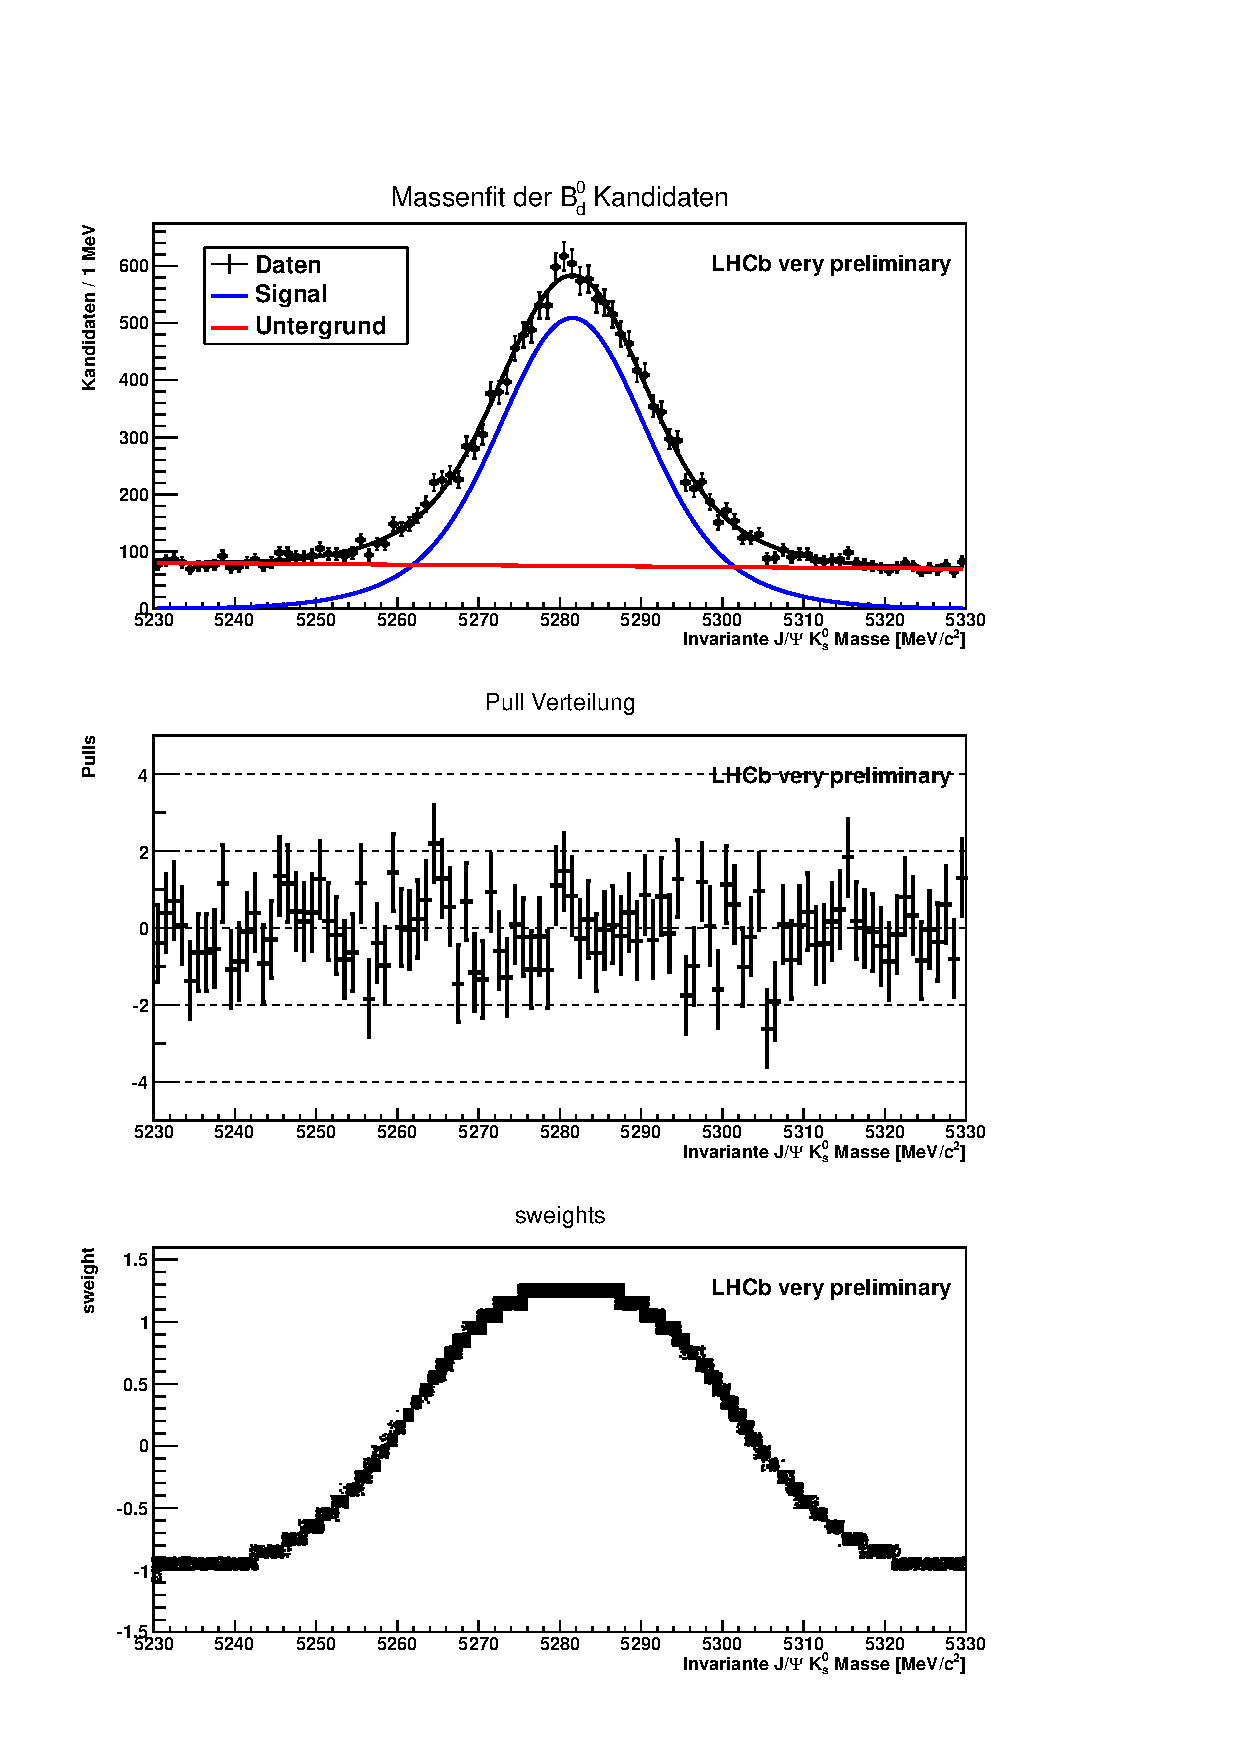
\includegraphics[width=\textwidth]{mass_fit}
\caption{Ergebnis des Massenfits}
\label{fig:fit_masse}
\end{figure}


\section{Wahrscheinlichkeitsdichtefunktion der Zerfallszeitverteilung}
In diesem Abschnitt soll nun die Wahrscheinlichkeitsdichtefunktion entwickelt werden, die letztendlich zur Bestimmung der Asymmetrie-Amplitude $\SJPsi$ verwendet wird. Aus den Gleichungen \ref{eq:bd} und \ref{eq:bdbar} geht für $|\lambda_f|=1$ die theoretische Zerfallszeitverteilung für ein \Bd bzw. \Bdbar hervor:
\begin{align}
\mathcal{P}_{\text{wahr}}(t, d_{\text{wahr}}) = \frac{1}{\mathcal{N}_t}\e^{-t/\tau}\left[1-d_{\text{wahr}}\SJPsi\sin(\sinarg)\right].
\end{align}
Durch die Einführung des wahren Tags $d_{\text{wahr}}$ wurden beide Verteilungen zu einer zusammengefasst. Ein anfängliches \Bd wird dabei durch $d_{\text{wahr}}=1$ beschrieben, ein \Bdbar durch $d_{\text{wahr}}=-1$. Die Normierung ist so gewählt, dass die Bedingung
\begin{align}
\sum_{d_{\text{wahr}}}\int_{t_{min}}^{t_{max}}\mathrm{d}t\mathcal{P}_{\text{wahr}}(t, d_{\text{wahr}}) = 1
\end{align}
erfüllt wird. Aufgrund zahlreicher detektorbedingten Effekte muss $\mathcal{P}_{\text{wahr}}(t, d_{\text{wahr}})$ modifiziert werden.

\subsection{Produktionsasymmetrie}
Der Detektor produziert \Bd- und \Bdbar-Mesonen nicht in exakt gleicher Zahl. Über die Produktionsraten $R_{\text{\Bdbar}}$ für ein \Bdbar bzw. $R_{\text{\Bd}}$ für ein \Bd ist die Produktionsasymmetrie definiert durch:
\begin{align}
\mu = A_P = \frac{R_{\text{\Bdbar}}-R_{\text{\Bd}}}{R_{\text{\Bdbar}}+R_{\text{\Bd}}}.
\end{align}
Anhand dieser Definition muss der Anteil an \Bd bzw. \Bdbar an der gesamten WDF gewichtet werden. Unter Verwendung des Kronecker-Deltas $\delta_{ij}$ lässt sich die WDF daher schreiben als:
\begin{align}
\nonumber \tilde{\mathcal{P}}_{\text{wahr}}(t, d_{\text{wahr}}) &= \delta_{d_{\text{wahr}},1}(1-\mu)\mathcal{P}_{\text{wahr}}(t, 1) + \delta_{d_{\text{wahr}},-1}(1+\mu)\mathcal{P}_{\text{wahr}}(t, -1) \\
\nonumber &= (1-d_{\text{wahr}}\mu)\mathcal{P}_{\text{wahr}}(t, d_{\text{wahr}}) \\
&= \frac{1}{\mathcal{N}_t}\e^{-t/\tau}\left[1-d_{\text{wahr}}\mu - (d_{\text{wahr}}-\mu)\SJPsi\sin(\sinarg)\right].
\end{align}

\subsection{Bestimmung des Anfangszustandes der \Bd-Mesonen(Tagging)}
\subsection{Zeitauflösung}
\subsection{Endgültige p.d.f.}
\begin{equation}
xxx     \label{eg:fit_pdf}
\end{equation}



\section{Fitergebnis} \label{kap:fitergebnis}
Wir erhalten schließlich:
\begin{align}
\SJPsi = xxx \pm xxx     \label{eq:fit_result}
\end{align}
\chapter{Abschätzung systematischer Unsicherheiten} \label{kap:systematik}
Der Fitter liefert zwar eine statistische Unsicherheit auf $\SJPsi$, allerdings ist eine Betrachtung der Systematik unerlässlich. Im Folgenden wird daher der Einfluss einiger Effekte auf das Fitergebnis untersucht und anschließend der systematische Fehler abgeschätzt.

\section{Fitmethode} \label{kap:fit_bias}
Es ist allgemein bekannt, dass die Parameterabschätzung der Maximum-Like\-li\-hood-Methode für eine große Zahl an Messwerten gegen den \glqq wahren Wert\grqq\ konvergiert, für wenig Statistik verfälscht sie jedoch das Ergebnis - sie produziert ein sogenanntes Bias. Um abzuschätzen, ob und in welchem Maße es zu einem Bias kommt, wird eine Toy Monte Carlo - Studie (kurz: Toy MC) durchgeführt. Dabei werden zufällig Daten der Massen- und Eigenzeit-WDF aus Gleichung (\ref{eq:pdf_masse}) bzw. (\ref{eq:fit_pdf}) folgend mit den gewünschten Parametern generiert und im Anschluss gefittet. Zur Generation der Massen- und Eigenzeitverteilung werden die aus den Fits erhaltenen Parameter verwendet (siehe Tabellen \ref{tab:fit_masse} und \ref{tab:fit_results}). Die einzige Ausnahme bildet $\SJPsi$, da diese zum Zeitpunkt dieser Studie noch verdeckt war. Hier wurde mit $\SJPsi = 0,72$, dem Resultat der Analyse aus 2011 \cite{lhcb-paper}, generiert. Entsprechend der Statistik im verwendeten Datensatz werden hier jeweils 20000 Ereignisse generiert. Durch mehrmaliges Wiederholen von Generation und Fit sollten die gefitteten Parameter am Ende mit der Größe des statistischen Fehlers gaußverteilt um die in der Generation verwendeten Parameter sein. Kommt es zu Abweichungen davon, so ist dies auf die Fitmethode oder eine fehlerhafte Implementation des Experimentators zurückzuführen. Um statistisch zuverlässige Aussagen treffen zu können, wurden in dieser Toy MC - Studie insgesamt 20000 Wiederholungen durchgeführt.

\begin{figure}[hptb]
\centering
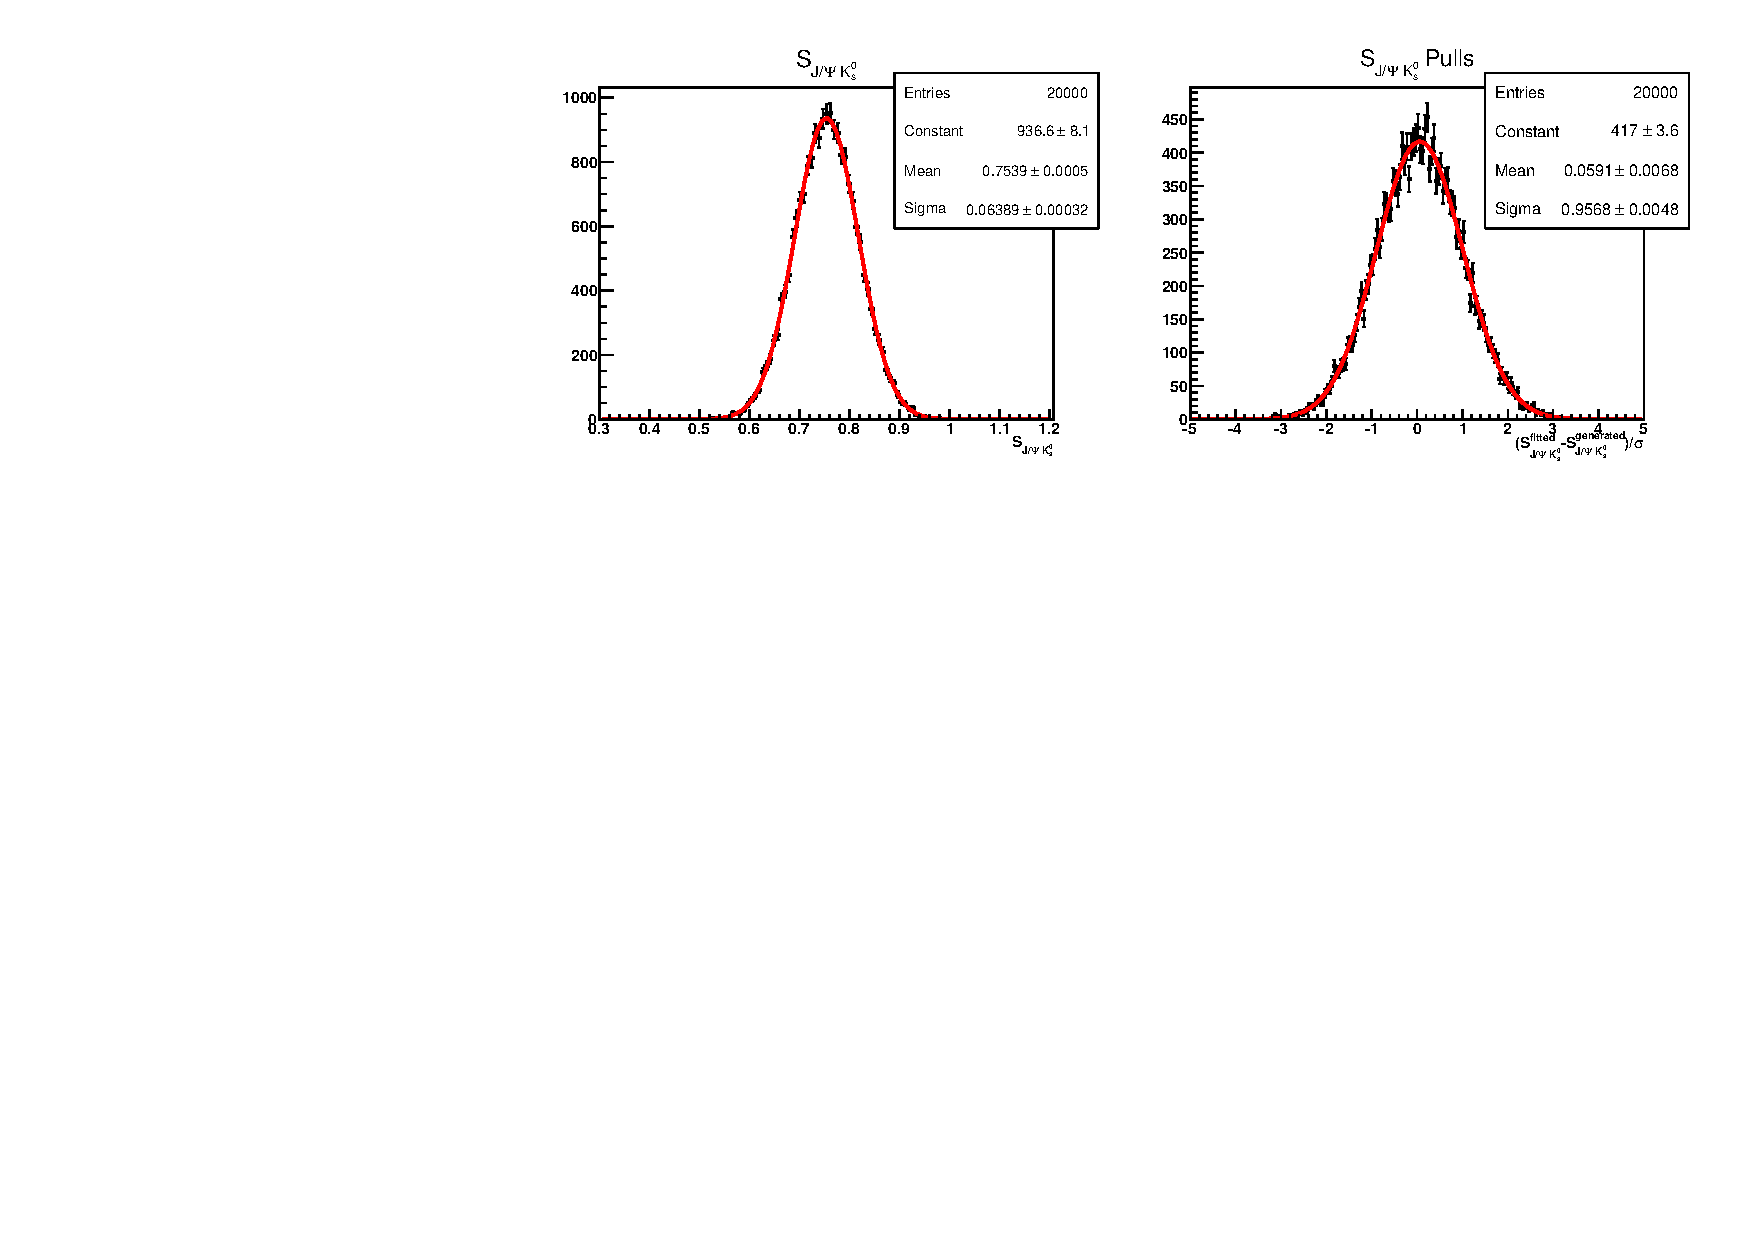
\includegraphics[width = \textwidth]{fit_bias}
\caption{Verteilung der aus der Toy MC Studie erhaltenen Amplituden $\SJPsi$ (links) sowie die dazugehörigen Pulls (rechts)}
\label{fig:fit_bias}
\end{figure}

Abbildung \ref{fig:fit_bias} zeigt sowohl die Verteilung der gefitteten Amplitude $\SJPsi$ als auch die Pulls, die sich mittels $(\SJPsi^{\text{gefittet}} - \SJPsi^{\text{generiert}})/\sigma^{\text{gefittet}}$ berechnen lassen. Der Mittelwert der Amplitudenverteilung (links) $\SJPsi^{\text{ToyMC}} = 0,7234 \pm 0,0004$ weicht signifikant vom generierten Wert $\SJPsi = 0,7200$ ab, es gibt also ein Bias. An der Pull-Verteilung lassen sich prinzipiell zwei Dinge beobachten:
\begin{enumerate}
    \item An der Verschiebung des Pull-Mittelwertes $\mu = 0,0522 \pm 0,0067$ von der Null sieht man deutlich, dass es - wie bereits erwähnt - ein kleines, aber signifikantes Bias gibt. Indem dieses Bias mit der statistischen Unsicherheit aus dem Fitergebnis (siehe Gl. (\ref{eq:fit_result})) multipliziert wird, erhält man eine Abschätzung der aus der Fitmethode resultierenden Unsicherheit:
        \begin{align}
        \delta\SJPsi^{Fit} = 0,0522 \cdot 0,0626 = 0,0033
        \end{align}

    \item Mit einem $\sigma = 0,941 \pm 0,005$ ist die Pull-Verteilung signifikant zu schmal. Bei einer zufälligen Streuung der Werte wird $\sigma=1$ erwartet. Dies bedeutet, dass der Fit den statistischen Fehler um $5,9\%$ überschätzt. Jenes Ergebnis kann später als Faktor zur Korrektur des statistischen Fehlers verwendet werden. 
\end{enumerate}

\subsubsection{Ursachen des Bias und der Fehlerüberschätzung}
Es bleibt zu klären, welche Ursachen zu dem Bias und der Fehlerüberschätzung führen. Wie bereits erwähnt, verfälscht die Likelihood-Methode für zu wenige Messwerte / Ereignisse die Parameterabschätzung. Demnach liegt die Vermutung nahe, dass im vorliegenden Datensatz zu wenig Ereignisse (\glqq Statistik\grqq) vorhanden sind. Daher wurden weitere Toy MC Studien mit unterschiedlicher Anzahl an generierten Teilchen pro Toy durchgeführt. Die Ergebnisse sind in Tabelle \ref{tab:fit_bias_events} aufgeführt und in Abbildung \ref{fig:fit_bias_events} nochmals visualisiert. Man sieht, dass das Bias mit erhöhter Statistik deutlich reduziert wird und damit zu wenig Statistik als Hauptursache hierfür angesehen werden kann.
\begin{table}[hptb]
\centering
\caption{Toy MC Studien mit unterschiedlicher Anzahl an generierten Ereignissen pro Toy. Genannt wird der Mittelwert $\mu$ der $\SJPsi$-Pull-Verteilung.}
\label{tab:fit_bias_events}
\begin{tabular}{cr@{$\pm$}l}
\hline \hline 
Teilchen pro Toy & \multicolumn{2}{c}{$\mu$}  \\ \hline
20000            &  0,0522 & 0,0067 \\
50000            &  0,0358 & 0,0067 \\
100000           &  0,0257 & 0,0068 \\
200000           &  0,0145 & 0,0068 \\ 
\hline \hline
\end{tabular}
\end{table}
\begin{figure}[hptb]
\centering
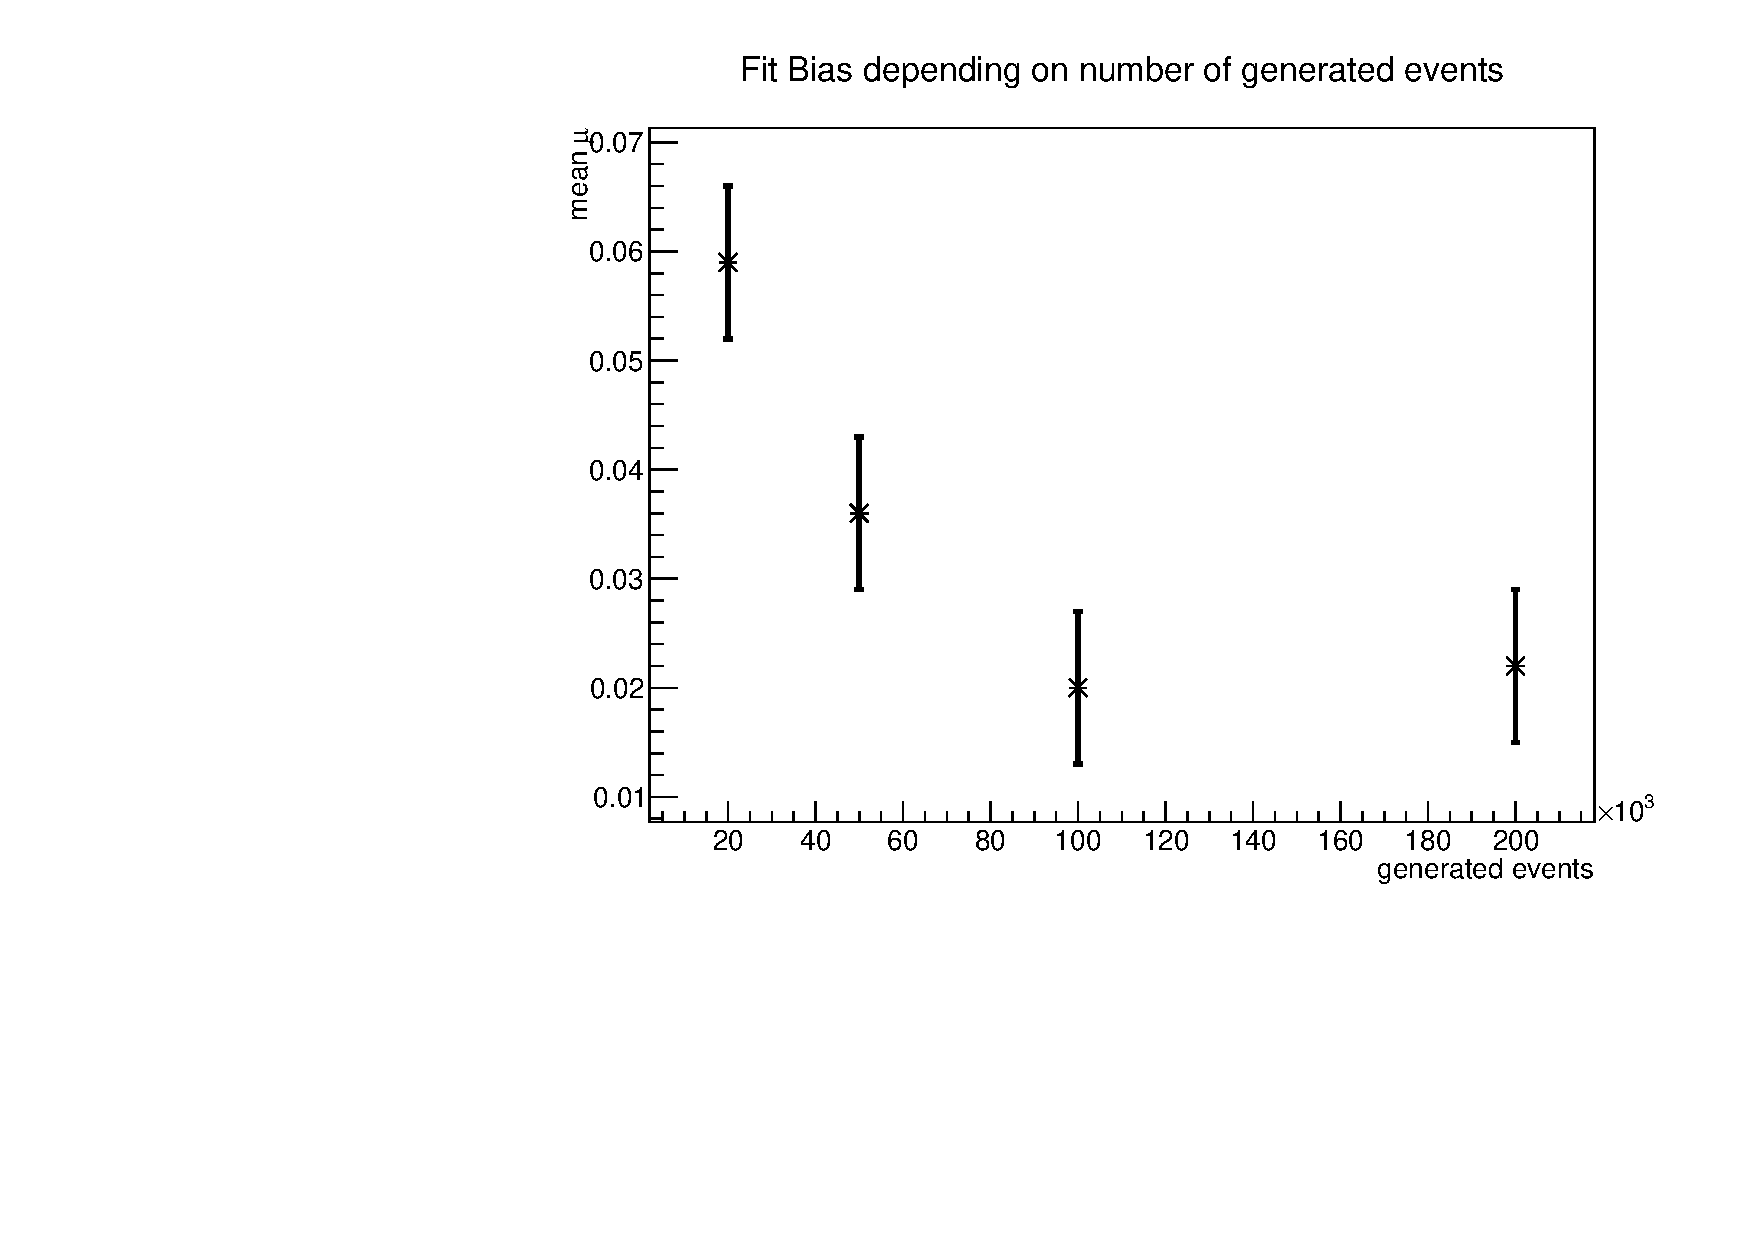
\includegraphics[width=\textwidth]{fit_bias_statistics}
\caption{Toy MC Studien mit unterschiedlicher Anzahl an generierten Ereignissen pro Toy. Als Maß für das Fit Bias dient der Mittelwert $\mu$ der $\SJPsi$-Pull-Verteilung. Der erste Eintrag entspricht der in Daten vorliegenden Statistik.}
\label{fig:fit_bias_events}
\end{figure}

Die Fehlerüberschätzung tritt auf, sobald man in den Toys Untergrund miteinbezieht (ohne Untergrund erhält man ein $\sigma=1,007\pm 0,005$ und ist damit kompatibel zur Eins). Es ist bekannt, dass die verwendete sFit-Methode die Fehlerpropagation (gerade bei Untergrund) nicht korrekt ausführt. Es wurde zuvor eine Fehlerkorrektur implementiert, dabei handelt es sich jedoch um eine Näherung. Für eine tiefergehende Studie müsste die Fehlerkorrektur entsprechend analysiert werden.

\section{Kalibration der Flavour Tagging Algorithmen} \label{kap:syst_tagging}
Im Fit werden bei den Parametern der Tagging Kalibration durch gaußische Einschränkung der Parameter deren statistische Fehler berücksichtigt. Bislang unbeachtet blieben die systematischen Fehler von $p_0$ und $p_1$, deren Einfluss im Folgenden untersucht wird. Leider sind die externen Studien zur Systematik des in dieser Analyse verwendeten Flavour Taggings noch nicht abgeschlossen, sodass die systematischen Fehler $\delta p_0^{\text{stat.}}$ sowie $\delta p_1^{\text{stat.}}$ noch nicht vorliegen. Um dennoch ein Gefühl für den Einfluss des Flavour Taggings zu bekommen, werden die systematischen Fehler der 2011-Analyse \cite{lhcb-paper} herangezogen. Die Annahme und Erwartung ist, dass sich die Systematiken zwischen 2011 und 2012 kaum unterscheiden. Für eine endgültige Analyse muss dieser Schritt jedoch wiederholt werden, sobald die Analyse des Flavour Taggings aus 2012 abgeschlossen ist. Eine weitere Möglichkeit wäre dann, die Parameter im Eigenzeitfit mit $\sigma = \sqrt{\sigma_{\text{stat.}}^2+\sigma_{\text{syst.}}^2}$ gaußisch einzuschränken und beide Unsicherheiten auf diese Weise zu berücksichtigen. In dieser Arbeit werden nun folgende Werte und Fehler der Kalibrationsparameter $p_0$ und $p_1$ verwendet:
\begin{align}
p_0 &= 0,382 \pm 0,003\ \text{(stat.)} \pm 0,008\ \text{(syst.)}, \\
p_1 &= 0,981 \pm 0,024\ \text{(stat.)} \pm 0,012\ \text{(syst.)}.
\end{align}

\subsubsection{Variation der Parameter in den Daten}
Einen ersten Überblick über die Systematik erhält man, indem man
im regulären Eigenzeitfit die Startwerte der Parameter $p_0$ und $p_1$ um ihre systematischen Fehler variiert. In allen vier möglichen Kombinationen wird der systematische Fehler auf $p_0$ und $p_1$ addiert bzw. subtrahiert, dann der Fit durchgeführt und schließlich die Abweichung vom regulären Fitergebnis für $\SJPsi$ berechnet. Der verdeckte Referenzwert aus dem Fit beträgt
\begin{align}
\SJPsi = 0,5347 \pm 0,0626.
\end{align}
\begin{table}[hptb]
\centering
\caption{Variation des Fitergebnisses für $\SJPsi$ bei Veränderung der Startwerte für $p_0$ und $p_1$ $\pm$ ihrer systematischen Unsicherheiten.}
\label{tab:syst_fit_calib_data}
$\begin{array}{cc|r@{\pm}l|r}
\hline\hline
p_0  &  p_1  &  \multicolumn{2}{c|}{\SJPsi}  & \Delta\SJPsi   \\ \hline
0,382 - 0,008  &  0,981 - 0,024  &  0,5109 & 0,0604  &  -0,0238 \\
0,382 - 0,008  &  0,981 + 0,024  &  0,5103 & 0,0604  &  -0,0244 \\
0,382 + 0,008  &  0,981 - 0,024  &  0,5599 & 0,0649  &   0,0252 \\
0,382 + 0,008  &  0,981 + 0,024  &  0,5591 & 0,0648  &   0,0244 \\
\hline\hline
\end{array}$
\end{table}
Die Ergebnisse sind Tabelle \ref{tab:syst_fit_calib_data} zu entnehmen. Die größte Abweichung beträgt hier $\Delta\SJPsi = 0,0252$.

\subsubsection{Variation der Parameter in Toy MC}
Eine präzisere Möglichkeit der Abschätzung besteht darin, sich entsprechende Toys mit verfälschten $p_0$ und $p_1$ zu generieren und diese dann normal zu fitten. Im Folgenden werden bei der Generation der Toys die Parameter $p_0$ und $p_1$ um ihre systematischen Unsicherheiten variiert, der Fit dann allerdings mit den ursprünglichen Parameterwerten durchgeführt. Als Referenzwert dient die Toy MC Studie aus Kapitel \ref{kap:fit_bias}, da dort mit den regulären Parametern $p_0$ und $p_1$ generiert und gefittet wurde. Jene Amplitude betrug
\begin{align}
\SJPsi = 0,7234 \pm 0,0004.
\end{align}
\begin{table}[hptb]
\centering
\caption{Variation des Fitergebnisses für $\SJPsi$ bei Veränderung der Parameterwerte $p_0$ und $p_1$ $\pm$ ihrer systematischen Unsicherheiten bei der Generation von Toys}
\label{tab:syst_fit_calib_toys}
$\begin{array}{cc|r@{\pm}l|r}
\hline\hline
p_0  &  p_1  &  \multicolumn{2}{c|}{\SJPsi}  & \Delta\SJPsi   \\ \hline
0,382 - 0,008  &  0,981 - 0,024  &  0,7515 & 0,0004  &   0,0281 \\
0,382 - 0,008  &  0,981 + 0,024  &  0,7565 & 0,0004  &   0,0331 \\
0,382 + 0,008  &  0,981 - 0,024  &  0,6909 & 0,0004  &  -0,0325 \\
0,382 + 0,008  &  0,981 + 0,024  &  0,6966 & 0,0004  &  -0,0244 \\
\hline\hline
\end{array}$
\end{table}

Die Ergebnisse sind Tabelle \ref{tab:syst_fit_calib_toys} zu entnehmen, die dazugehörigen Plots werden in Abbildung \ref{fig:toys_tag_calib} gezeigt. Die größte Abweichung beträgt hier $\Delta\SJPsi = 0,0331$ und ist auch größer als bei Variation der Parameter in den Daten. Dementsprechend wird der systematische Fehler durch die Flavour Tagging Kalibration mit ebendiesem Wert konservativ abgeschätzt:
\begin{align}
\delta\SJPsi^{\text{FTK}} = 0,0331.
\end{align}
\begin{figure}[hptb]
\centering
\subfigure[{$p_0 - \Delta p_0$,  $p_1 - \Delta p_1$}]{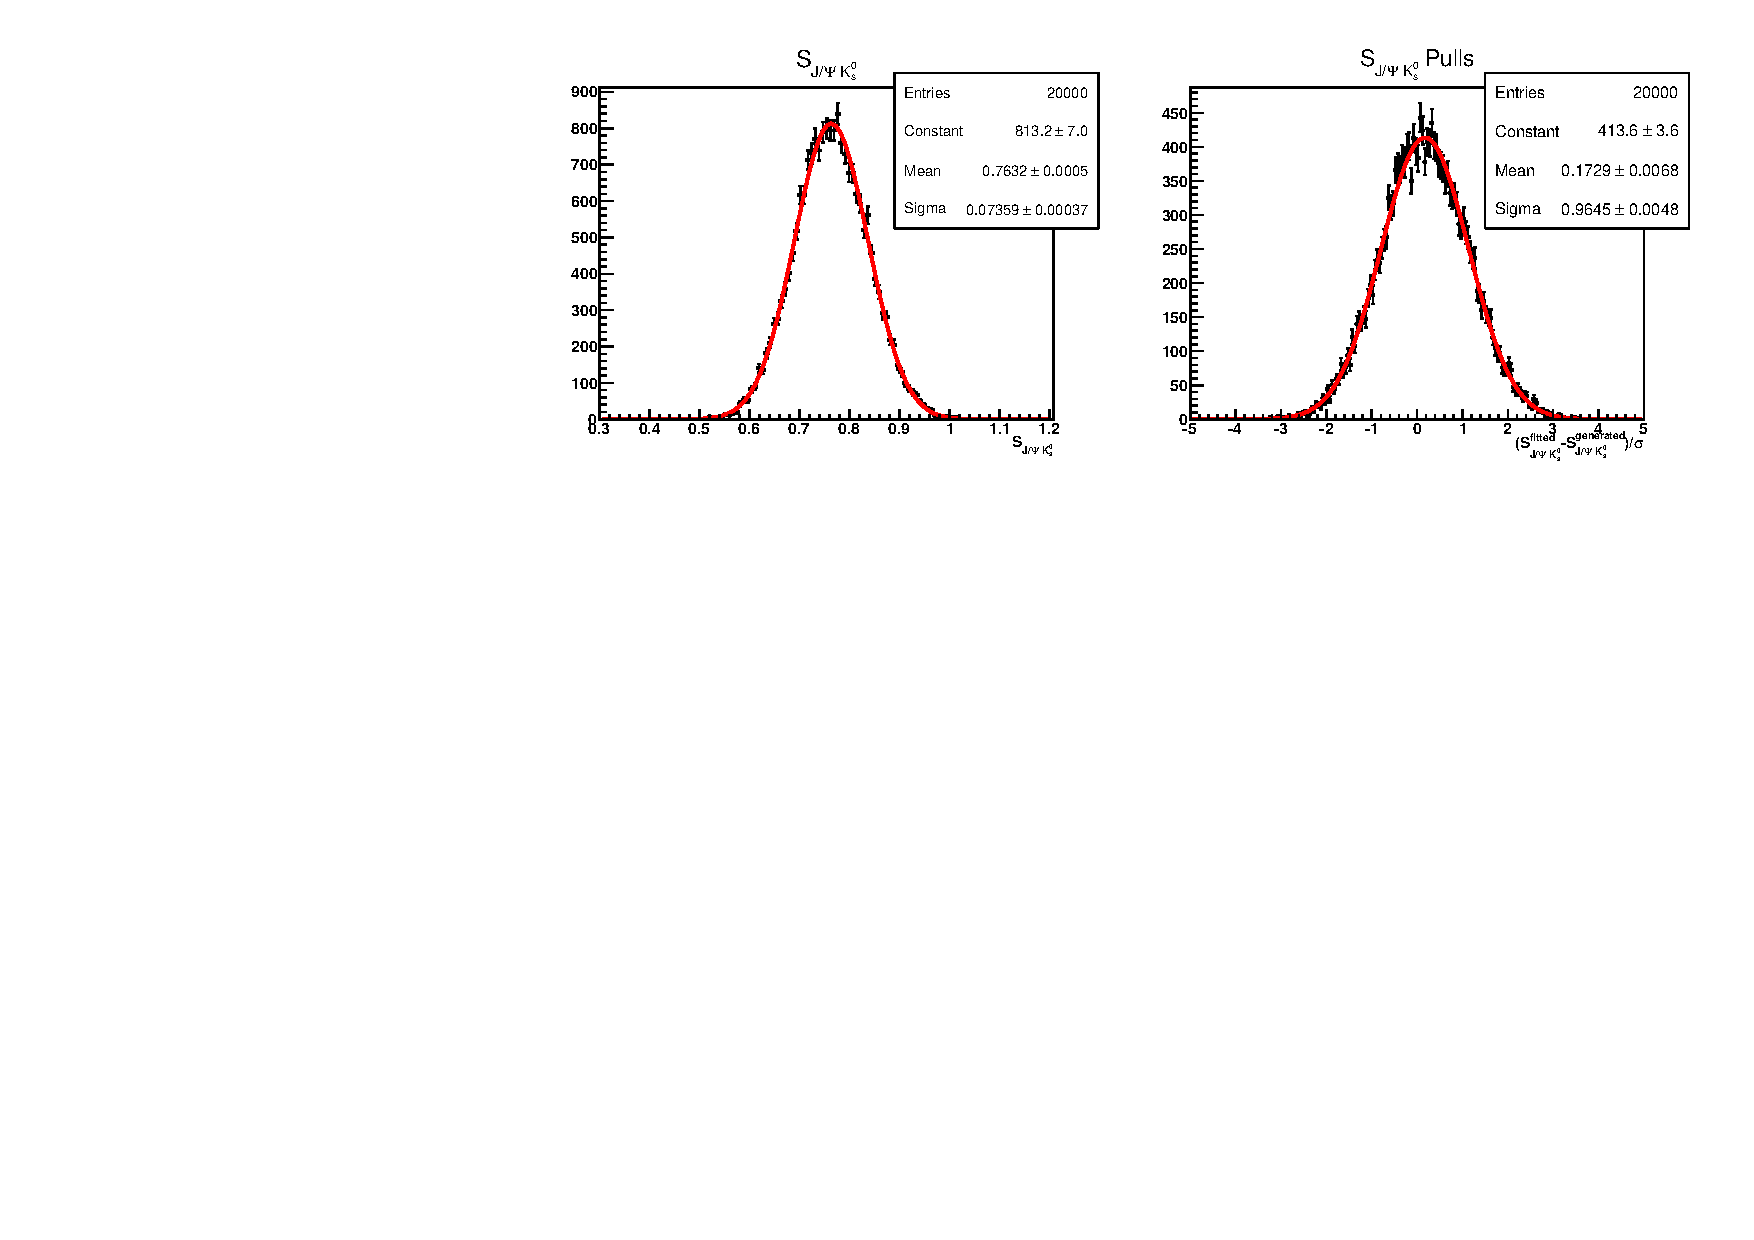
\includegraphics[width=0.75\textwidth]{tagging_calibration--}}
\subfigure[{$p_0 + \Delta p_0$,  $p_1 - \Delta p_1$}]{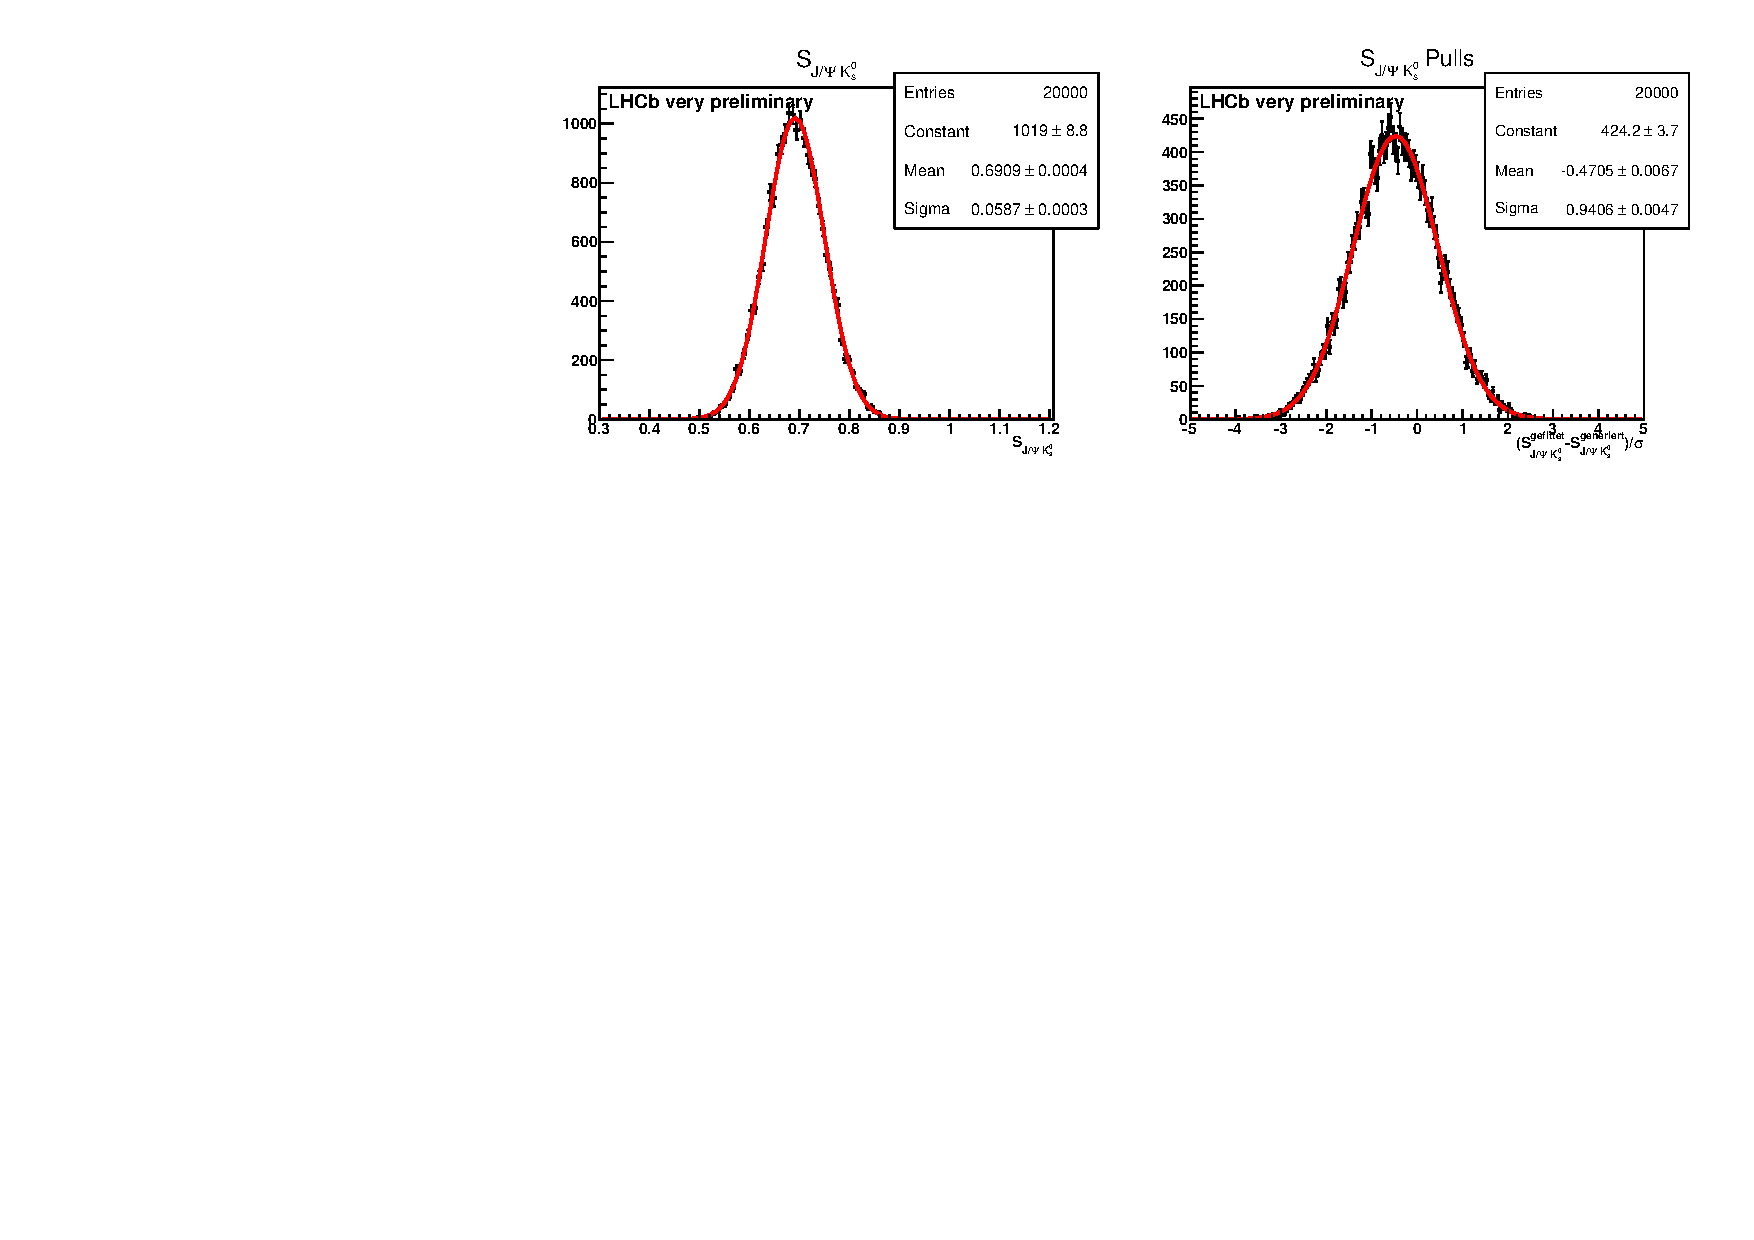
\includegraphics[width=0.75\textwidth]{tagging_calibration+-}}
\subfigure[{$p_0 - \Delta p_0$,  $p_1 + \Delta p_1$}]{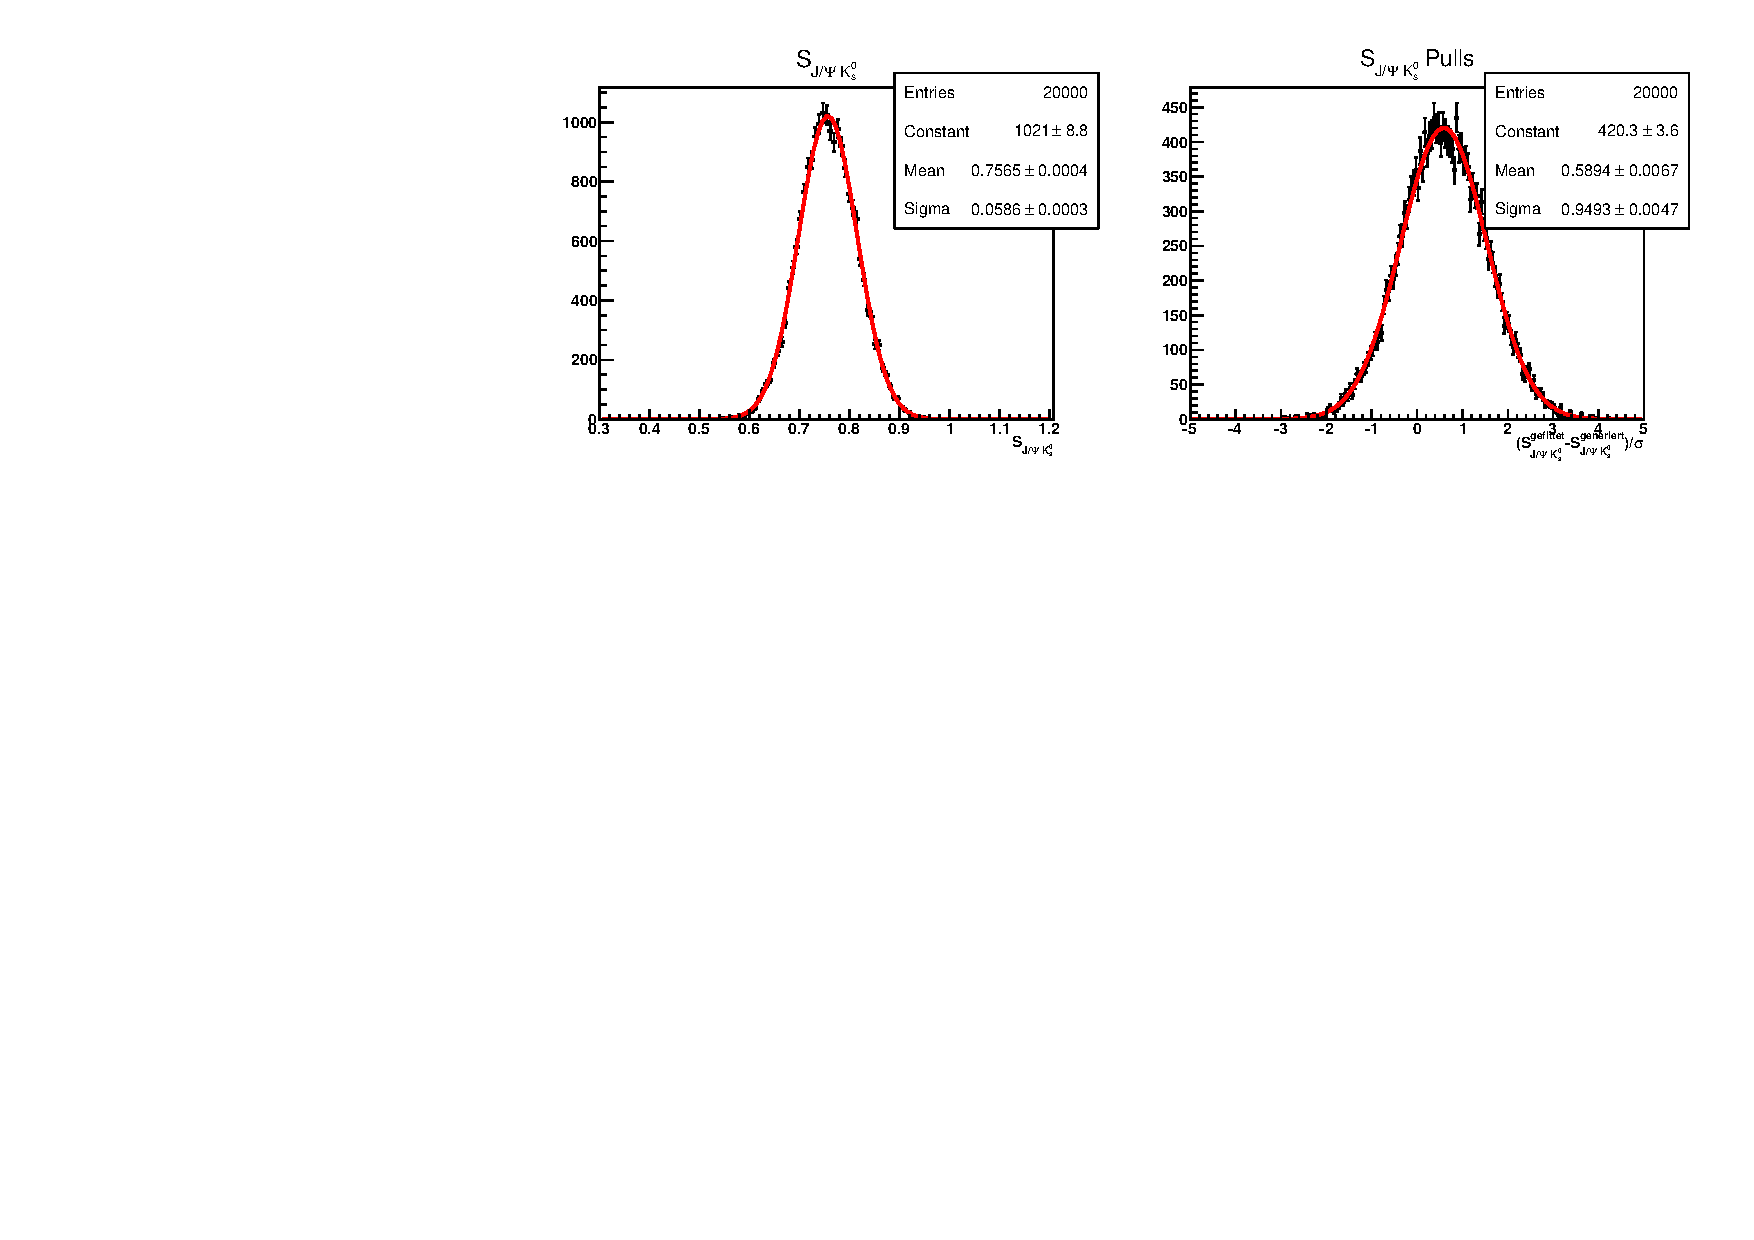
\includegraphics[width=0.75\textwidth]{tagging_calibration-+}}
\subfigure[{$p_0 + \Delta p_0$,  $p_1 + \Delta p_1$}]{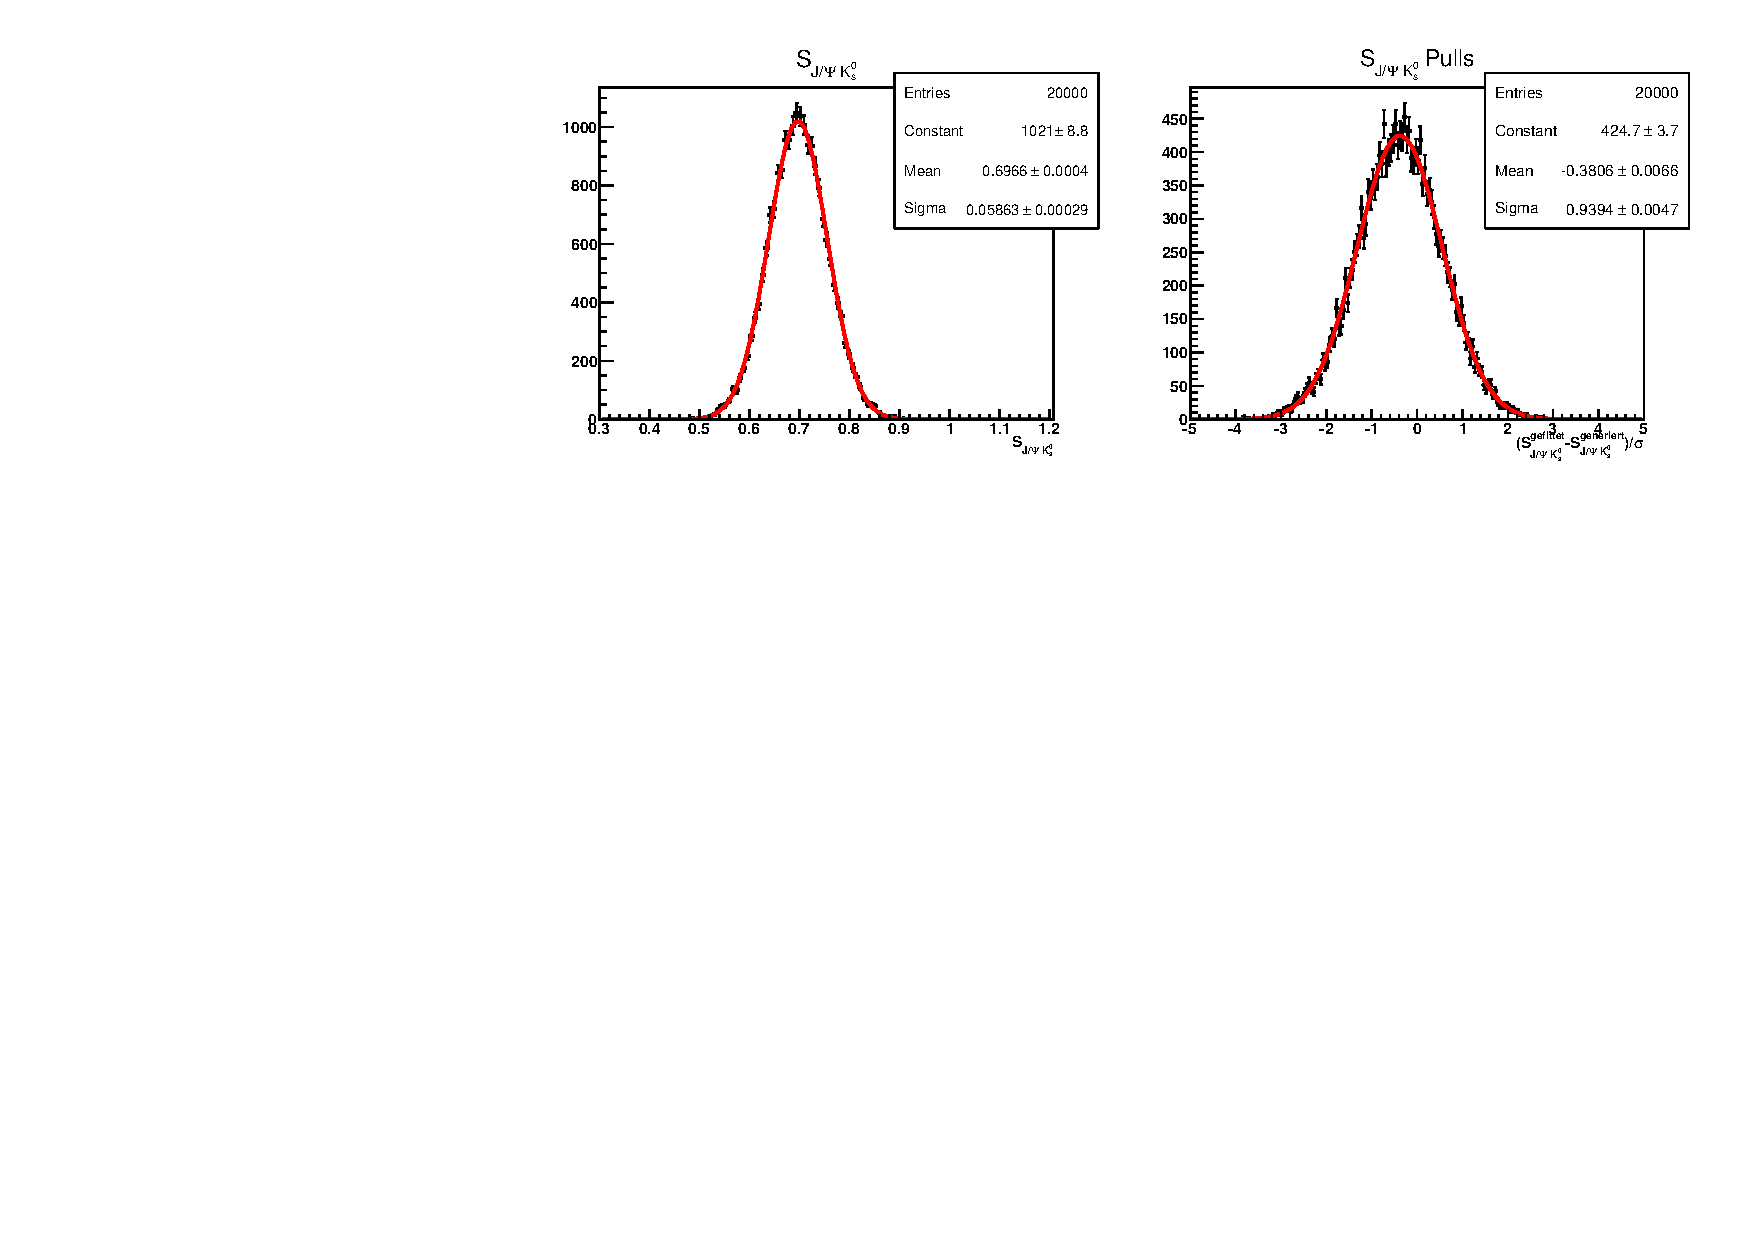
\includegraphics[width=0.75\textwidth]{tagging_calibration++}}
\caption{Toy MC Studie zur Abschätzung der Systematik durch die Tagging Kalibration. Bei der Generation wurden die Taggingparameter $p_0=0,382$ und $p_1=0,981$ um ihre systematischen Unsicherheiten $\Delta p_0 = 0,008$ bzw. $\Delta p_1 = 0,024$ variiert, der Fit wurde dann mit den ursprünglichen Werten $p_0$ und $p_1$ durchgeführt.}
\label{fig:toys_tag_calib}
\end{figure}

\section{Einfluss einer zeitabhängigen Akzeptanz} \label{kap:akzeptanz}
In der Analyse wurde der Einfluss einer zeitabhängigen Detektorakzeptanz vernachlässigt. Nimmt man an, dass sich die Akzeptanz von \Bd- und \Bdbar-Mesonen nicht unterscheiden, so hat die Akzeptanz keinen Einfluss auf die \CP-Asymmetrie nach Gleichung (\ref{eq:cp_asymm}), da sie sich hier herauskürzt. Beim Fit der Amplitude nach Gleichung (\ref{eq:fit_pdf}) ist dies aber nicht zwangsläufig der Fall. Um die Vernachlässigung einer zeitabhängigen Akzeptanz zu rechtfertigen, wird zunächst eine Bestimmung der Akzeptanz durchgeführt und anschließend mit einer Toy MC Studie ihr Einfluss überprüft.

\subsubsection{Bestimmung einer Akzeptanzfunktion} 
\Bd-Mesonen haben eine relativ lange Lebensdauer. Um sie von kurzlebigem Untergrund zu unterscheiden, befinden sich auf den Triggern und dem Stripping entsprechende Selektionen auf die Signifikanz der Zerfallslänge. Dies hat zur Folge, dass für kleine Flugzeiten ($t \lesssim 0,3\pico\second$) kaum \Bd-Mesonen im Detektor registriert werden. Es hat sich herausgestellt \cite{lhcb-paper}, dass dieser Effekt gut durch die Funktion
\begin{align}
\epsilon_1(t) = \frac{2}{\pi}\arctan[t\cdot \exp(at+b)]
\end{align}
parametrisiert werden kann. Je länger ein \Bd-Meson lebt, desto schwieriger wird es, diese Zerfallsprodukte im Detektor auf Grund seiner Geometrie nachzuweisen. Daher nimmt die Akzeptanz zu großen Zeiten hin wieder ab. Zur Parametrisierung fällt die Wahl auf eine lineare Funktion
\begin{align}
\epsilon_2(t) = 1 + \beta t \qquad (\beta < 0).
\end{align}
Die entsprechende gesamte Akzeptanzfunktion lautet demnach:
\begin{align}
\epsilon(t) = \epsilon_1(t) \cdot \epsilon_2(t) = \frac{2}{\pi}\arctan[t\cdot \exp(at+b)](1 + \beta t)
\end{align}
Zur Bestimmung der Parameter wird die Trennung von \Bd- und \Bdbar-Mesonen aufgehoben, sodass lediglich ein exponentieller Zerfall zu beobachten ist. Des weiteren wird die Selektion der Lebensdauer bei $0,3\pico\second$ nicht angewandt, sodass die Akzeptanz bei kleinen Eigenzeiten sichtbar wird. Die Wahrscheinlichkeitsdichtefunktion für den Fit lautet somit:
\begin{align}
\mathcal{P}_{acc}(t) \propto \epsilon(t)\cdot \e^{-t/\tau} = \e^{-t/\tau}\cdot\frac{2}{\pi}\arctan[t\cdot \exp(at+b)](1 + \beta t)
\end{align}
Die beiden Parameter $\tau$ und $\beta$ sind stark miteinander korreliert. Für eine geeignete Bestimmung der Parameter der Akzeptanz-Funktion wird daher die Lebensdauer auf den PDG-Wert $\tau = (1,519 \pm 0,007)\pico\second$ \cite{pdg-tau} gaußisch eingeschränkt, die anderen Parameter sind frei. Die Ergebnisse sind in Tabelle \ref{tab:fit_akzeptanz} aufgeführt, die entsprechenden Plots in Abbildung \ref{fig:fit_akzeptanz}. 
\begin{table}[hptb]
\centering
\caption{Ergebnis des Fits zur Bestimmung der zeitlichen Akzeptanz. $\tau$ wurde auf den PDG-Wert $\tau = (1,519 \pm 0,007)\pico\second$ \cite{pdg-tau} gaußisch eingeschränkt.}
\label{tab:fit_akzeptanz}
$\begin{array}{llr@{\pm}l}
\hline \hline 
\multicolumn{2}{l}{\text{Parameter}} & \multicolumn{2}{c}{\text{Ergebnis}}  \\ \hline
\tau  & [\ps]  &  1,519 & 0,007 \\
a   & [\ps]  &  47,9    & 5,6 \\
b   & &  -8,4    & 1,1 \\
\beta & [\ps^{-1}]  & -0,0090 & 0,0076 \\ 
\hline \hline
\end{array}$
\end{table}
\begin{figure}[hptb]
\centering
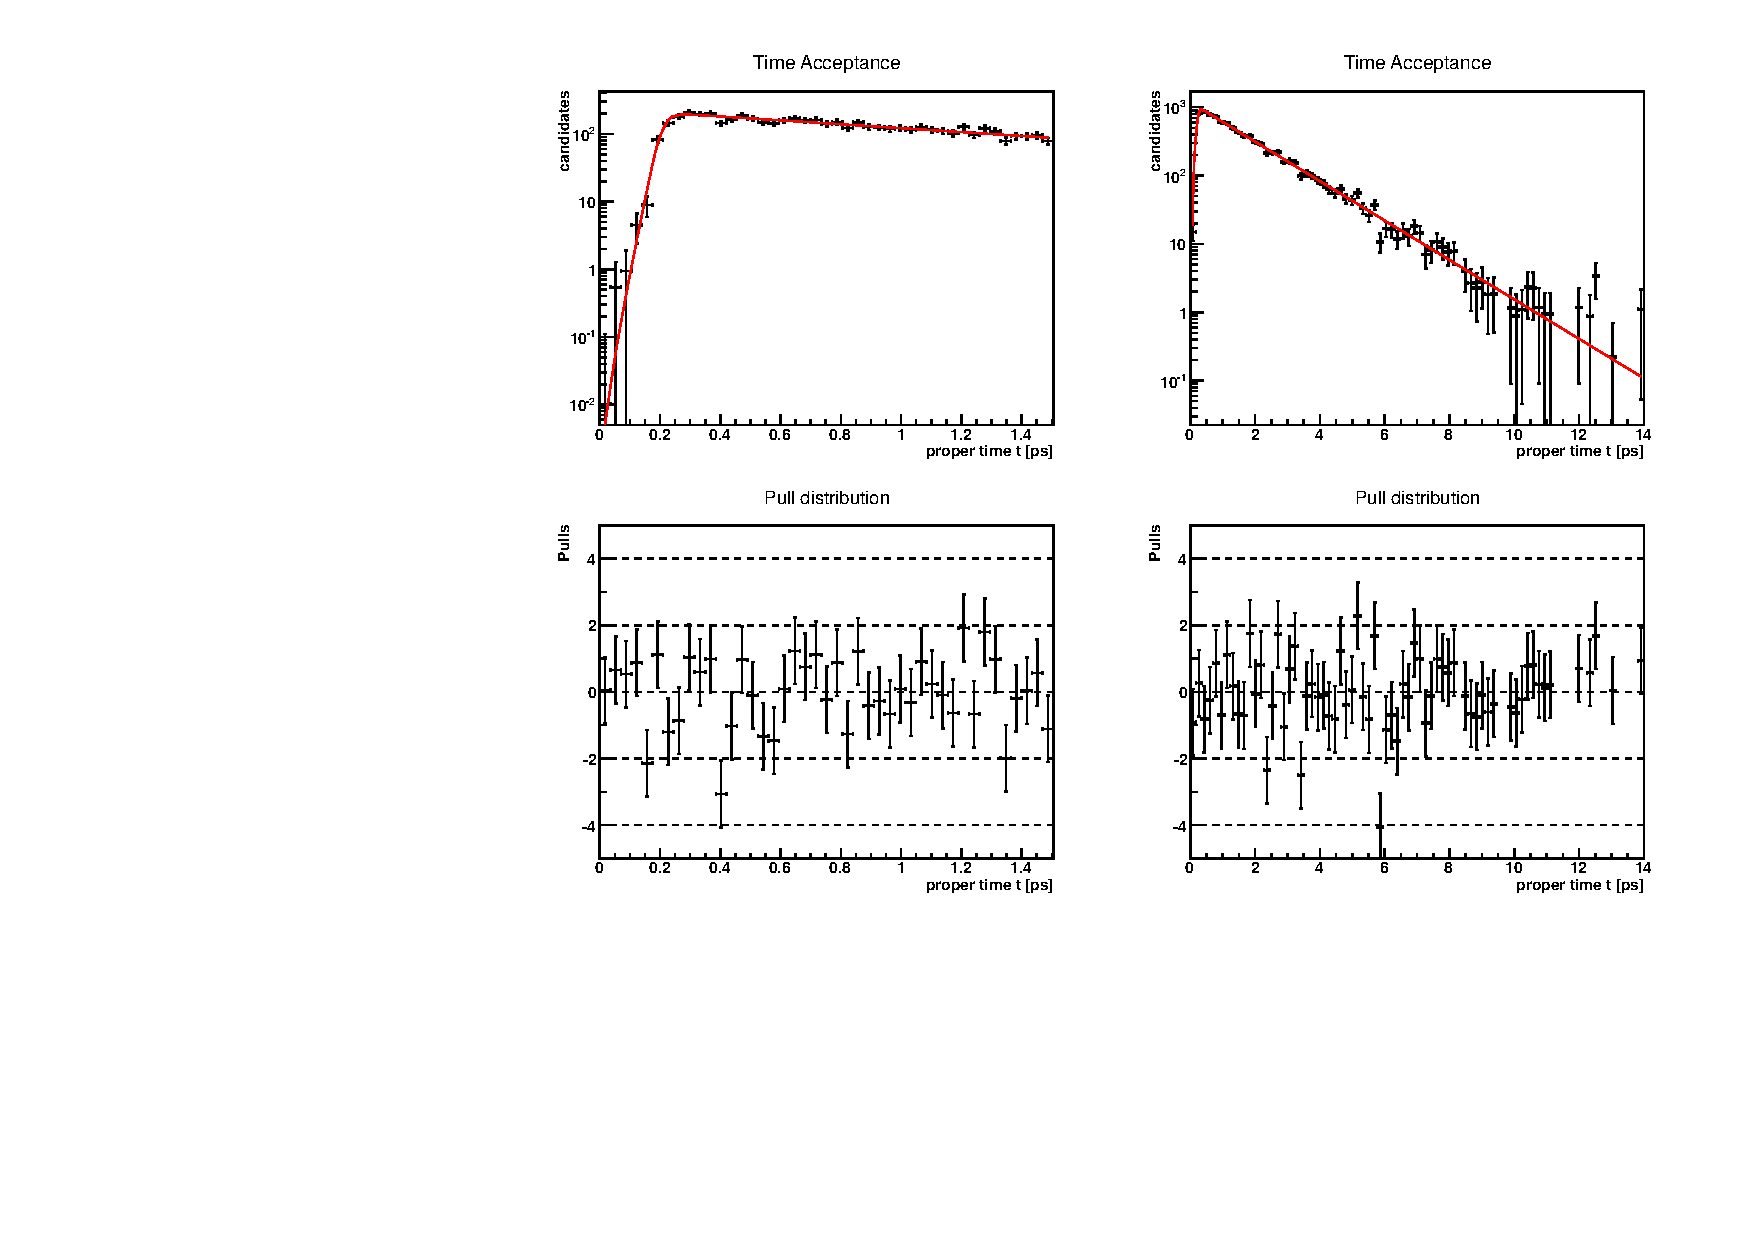
\includegraphics[width=\textwidth]{time_acceptance_fit}
\caption{Fit an die Eigenzeit-Verteilung aller \Bd-Mesonen mit eingeschlossener Akzeptanzfunktion (oben) sowie die entsprechende Pull-Verteilung (unten). Links: kurzlebiger Zeitbereich ($t<1,5\pico\second$), Rechts: gesamtes Eigenzeitspektrum ($0\ps < t < 14\ps$).}
\label{fig:fit_akzeptanz}
\end{figure}

\subsubsection{Bestimmung des Einflusses}
Durch die Selektion der Eigenzeit ab $t = 0,3\ps$ in der Datenselektion spielt die Akzeptanz für kleine Eigenzeiten kaum eine Rolle Dies wird dadurch deutlich, dass die Akzeptanzfunktion $\epsilon(0,3\ps) = 0,992$ und damit fast Eins ist. In der Analyse aus 2011 \cite{lhcb-paper} wurde nur ein geringer Effekt auf das Fitergebnis beobachtet. Dies soll nun verifiziert und das Vorgehen, im Eigenzeitfit die zeitliche Detektorakzeptanz zu vernachlässigen, gerechtfertigt werden. Mit den oben bestimmten Parametern wird die zeitliche Akzeptanz bei der Erzeugung von Daten einer weiteren Toy MC Studie berücksichtigt, der anschließende Fit aber ohne Akzeptanzfunktion durchgeführt. Die zur Erzeugung verwendeten Parameter entsprechen ansonsten denen in Kapitel \ref{kap:fit_bias}.
\begin{figure}[hptb]
\centering
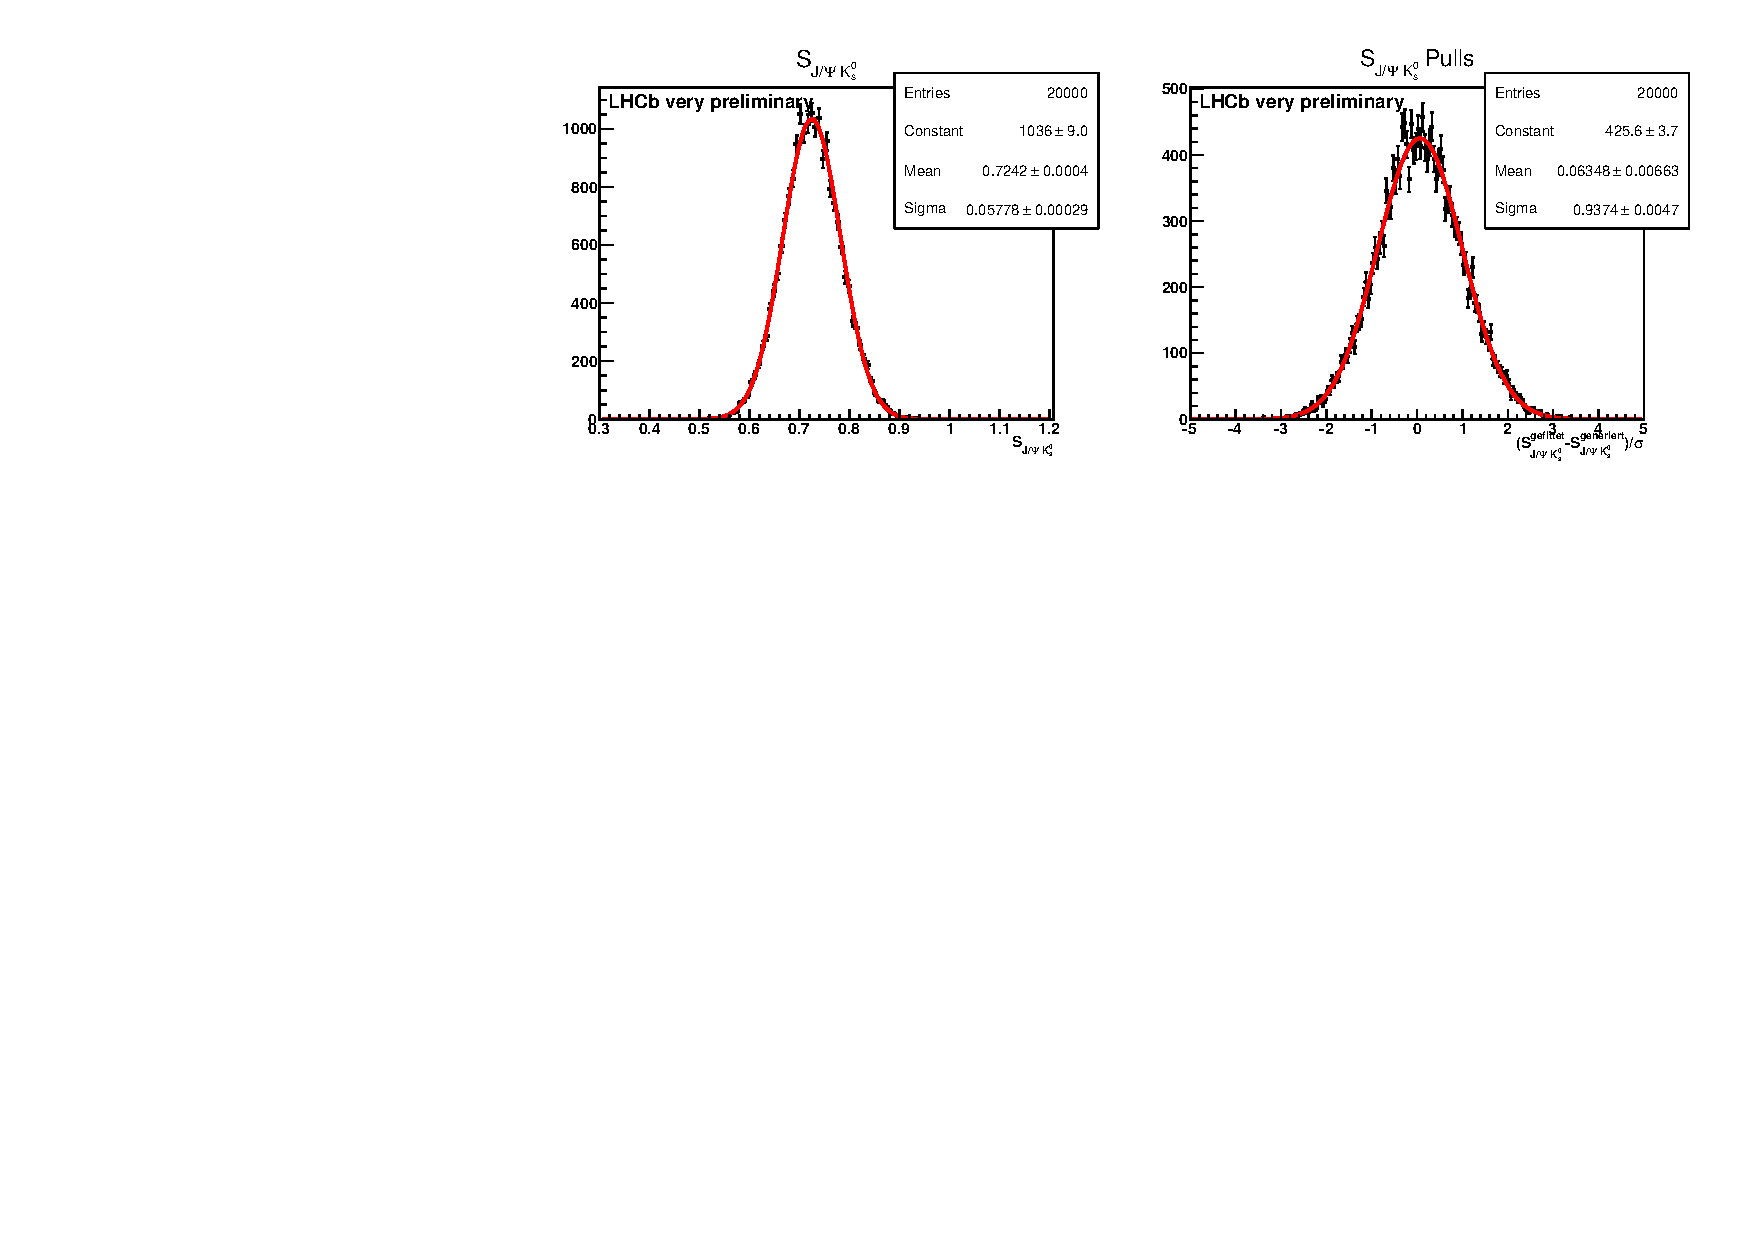
\includegraphics[width = \textwidth]{time_acceptance_toys}
\caption{Untersuchung des Einflusses einer zeitlichen Akzeptanz: Verteilung der aus der Toy MC Studie erhaltenen Amplituden $\SJPsi$ (links) sowie die dazugehörigen Pulls (rechts).}
\label{fig:toys_acceptance}
\end{figure}

Der Mittelwert der Amplitudenverteilung beträgt $\SJPsi = 0,72420 \pm 0,00041$. Die Abweichung vom Referenzwert $\SJPsi = 0,72343 \pm 0,00041$ (siehe Kap. \ref{kap:fit_bias}),
\begin{align}
\delta\SJPsi^{\text{Akz.}} = 0,00077\ ,
\end{align}
wird zur Abschätzung des Fehlers durch Vernachlässigung einer Akzeptanzfunktion verwendet. Gerade im Vergleich zum Einfluss des Flavour Taggings auf $\SJPsi$ ist dieser hier sehr gering. Somit erscheint das Vorgehen, keine Akzeptanz im Eigenzeitfit zu verwenden, gerechtfertigt.


\section{Korrelation zwischen Masse und Eigenzeit}
Die sFit-Methode funktioniert dann am besten, wenn das Signal und der Untergrund der Massenverteilung vollkommen unkorreliert zur Signal- und Untergrundverteilung der Eigenzeit ist. Es soll nun eine etwaige Korrelation zwischen Masse und Eigenzeit untersucht und der Einfluss auf $\SJPsi$ festgestellt werden. Dazu wird die Massenverteilung in vier verschiedenen Zeitbereichen gefittet, die Tabelle \ref{tab:mass_ct} zu entnehmen sind. Anschließend wird die gesamte Eigenzeitverteilung gefittet, dabei werden aber die Massenparameter auf die in den 4 Massenfits erhaltenen Werte fixiert. Die Ergebnisse des jeweiligen Fits sind ebenfalls in Tabelle \ref{tab:mass_ct} aufgeführt.
\begin{table}[hptb]
\centering
\caption{Einteilung der Eigenzeitbereiche sowie Fitresultate für $\SJPsi$ bei Fixierung der Masse auf die in den Zeitbereichen enthaltene Massenform. Weiterhin werden die Abweichung $\Delta\SJPsi$ vom regulären Datenfit und der Signalanzahl $N_{sig}$ eines jeden Eigenzeitbereichs genannt.}
\label{tab:mass_ct}
\begin{tabular}{c l r@{$\pm$}l c c}
\hline \hline
Nr. & Eigenzeitfenster des Massenfits & \multicolumn{2}{c}{$\SJPsi$} & $\Delta\SJPsi$ & $N_{sig}$\\ \hline
1 & $t \in [0,3; 0,7] \pico\second$ & 0,5318 & 0,0626 & -0,0029 & 2882 \\
2 & $t \in [0,7; 1,5] \pico\second$ & 0,5361 & 0,0625 & 0,0014 & 4066 \\
3 & $t \in [1,5; 3] \pico\second$ & 0,5361 & 0,0625 & 0,0014 & 4230 \\
4 & $t \in [3; 14] \pico\second$ & 0,5353 & 0,0624 & 0,0006 & 2177 \\ \hline \hline
\end{tabular}
\end{table}

Zur Abschätzung des Fehlers werden zunächst die Abweichungen $\Delta\SJPsi$ vom (noch verdeckten) Referenzwert aus dem regulären Eigenzeitfit $\SJPsi = 0,5347 \pm 0,0626$ berechnet (siehe Kap. \ref{kap:fitergebnis}) und diese dann - gewichtet nach der Signalzahl $N_{sig}$ eines jeden Bereichs - quadratisch gemittelt:
\begin{align}
\delta\SJPsi^{m/t} = \sqrt{\frac{\sum N_i (\Delta\SJPsi)_i^2}{\sum N_i}} = 0,0018
\end{align}

\section{Eigenzeitauflösung} \label{kap:aufloesung}
Bei einer effektiven Eigenzeitauflösung von $\sigma_{\text{eff}} = (0,0665 \pm 0,0013)\ps$ im Vergleich zur \Bd-Oszillationsfrequenz $\Delta m_d = (0,521 \pm 0.039)\ps$ erwartet man keine nennenswerten Effekte auf die Amplitude $\SJPsi$. Um überhaupt einen Effekt zu sehen, werden die Auflösungsparameter $\sigma_i$ um 20\% ihres Werte erhöht bzw. gesenkt und damit dann der Datensatz gefittet. Die größte Abweichung vom Referenzwert des regulären Eigenzeitfits wird als systematischer Fehler angenommen. Die Ergebnisse finden sich in Tabelle \ref{tab:syst_resolution}.

\begin{table}[hptb]
\centering
\caption{Ergebnisse des Eigenzeitfits bei Variaton der Auflösungsparameter $\sigma_i$ um $\pm 20\%$.}
\label{tab:syst_resolution}
\begin{tabular}{l c c c r@{$\pm$}l r }
\hline \hline
Variation & $\sigma_1$ & $\sigma_2$ & $\sigma_3$ & \multicolumn{2}{c}{$\SJPsi$} & $\Delta\SJPsi$ \\ \hline
$+20\%$ & 0,576 & 0,05275 & 0,1118 & 0,5351 & 0,0626 & 0,0004 \\
$-20\%$ & 0,384 & 0,03517 & 0,0746 & 0,5345 & 0,0625 & -0,0002 \\ \hline \hline
\end{tabular}
\end{table}
Es zeigt sich, dass eine exakte Bestimmung der Auflösung nicht von Nöten ist, da sie im Vergleich zu anderen Systematiken vor allem gegenüber der Flavour Tagging Kalibration vernachlässigt werden kann. Dennoch wird ein sytematischer Fehler durch die Auflösung mit
\begin{align}
\delta\SJPsi^{\text{Res.}} = 0,0004
\end{align}
assoziiert.

\section{Gesamtsystematik}
Tabelle \ref{tab:syst_gesamt} fasst nochmals alle systematischen Unsicherheiten zusammen. Der Gesamtfehler wird durch quadratische Addition berechnet.
\begin{table}[hptb]
\centering
\caption{Zusammenfassung der systematischen Unsicherheiten}
\label{tab:syst_gesamt}
\begin{tabular}{l c }
\hline \hline
Effekt & $\delta\SJPsi$ \\ \hline
Fitmethode & 0,0033 \\
Flavour Tagging Kalibration & 0,0331 \\
Eigenzeitakzeptanz & 0,0008 \\
Korrelation Masse $\leftrightarrow$ Eigenzeit & 0,0018 \\ 
Eigenzeitauflösung & 0,0004 \\ \hline 
Gesamt & 0,0333 \\ \hline \hline
\end{tabular}
\end{table}

Es ist deutlich zu erkennen, dass die Kalibration der Flavour Tagging Algorithmen die dominierende Systematik ist. Obwohl hier zur Abschätzung der Systematik Werte der 2011-Kalibration genommen werden mussten, wird sich an dieser Tatsache nicht viel ändern, sobald diese Untersuchung mit Werten aus 2012 wiederholt wurde. Der systematische Fehler von $\delta\SJPsi^{\text{stat.}}=0,0333$ ist nur etwa halb so groß wie der statistische $\delta\SJPsi^{\text{syst.}}=0,0626$. Damit ist definitiv noch Potential da, die Präzision durch mehr Datennahme zu verbessern. Zudem ist auch zu erwarten, dass die systematischen Unsicherheiten der Flavour Tagging Kalibration mit mehr Daten ebenfalls reduziert wird.
\chapter{Zusammenfassung}
In dieser Arbeit wurde die Amplitude der \CP-Asymmetrie $\SJPsi$ gemessen. Es wurde dabei die sFit-Methode angewandt, um Signal vom Untergund zu extrahieren. Dazu diente ein Fit der rekonstruierten \Bd-Masse. Aus dem anschließenden Fit der Eigenzeitverteilung erhält man
\begin{align}
\SJPsi = \sin(2\beta) = 0,711 \pm 0,059 (\text{stat.}) \pm 0,033 (\text{syst.})
\end{align}
Hierbei soll erwähnt werden, dass der statistische Fehler auf Grund der Erkenntnisse aus Kapitel \ref{kap:fit_bias} um den Faktor $\sigma_{\text{pull}} = 0,941$ korrigiert wurde. Das Ergebnis ist kompatibel zum Weltmittelwert $\sin(2\beta) = 0,682 \pm 0,019$ \cite{pdg-average} sowie zur LHCb-Analyse aus 2011 $\sin(2\beta) = 0.72 \pm 0,07 (\text{stat.}) \pm 0,04 (\text{syst.})$ \cite{lhcb-paper}. 

\begin{figure}[hptb]
\centering
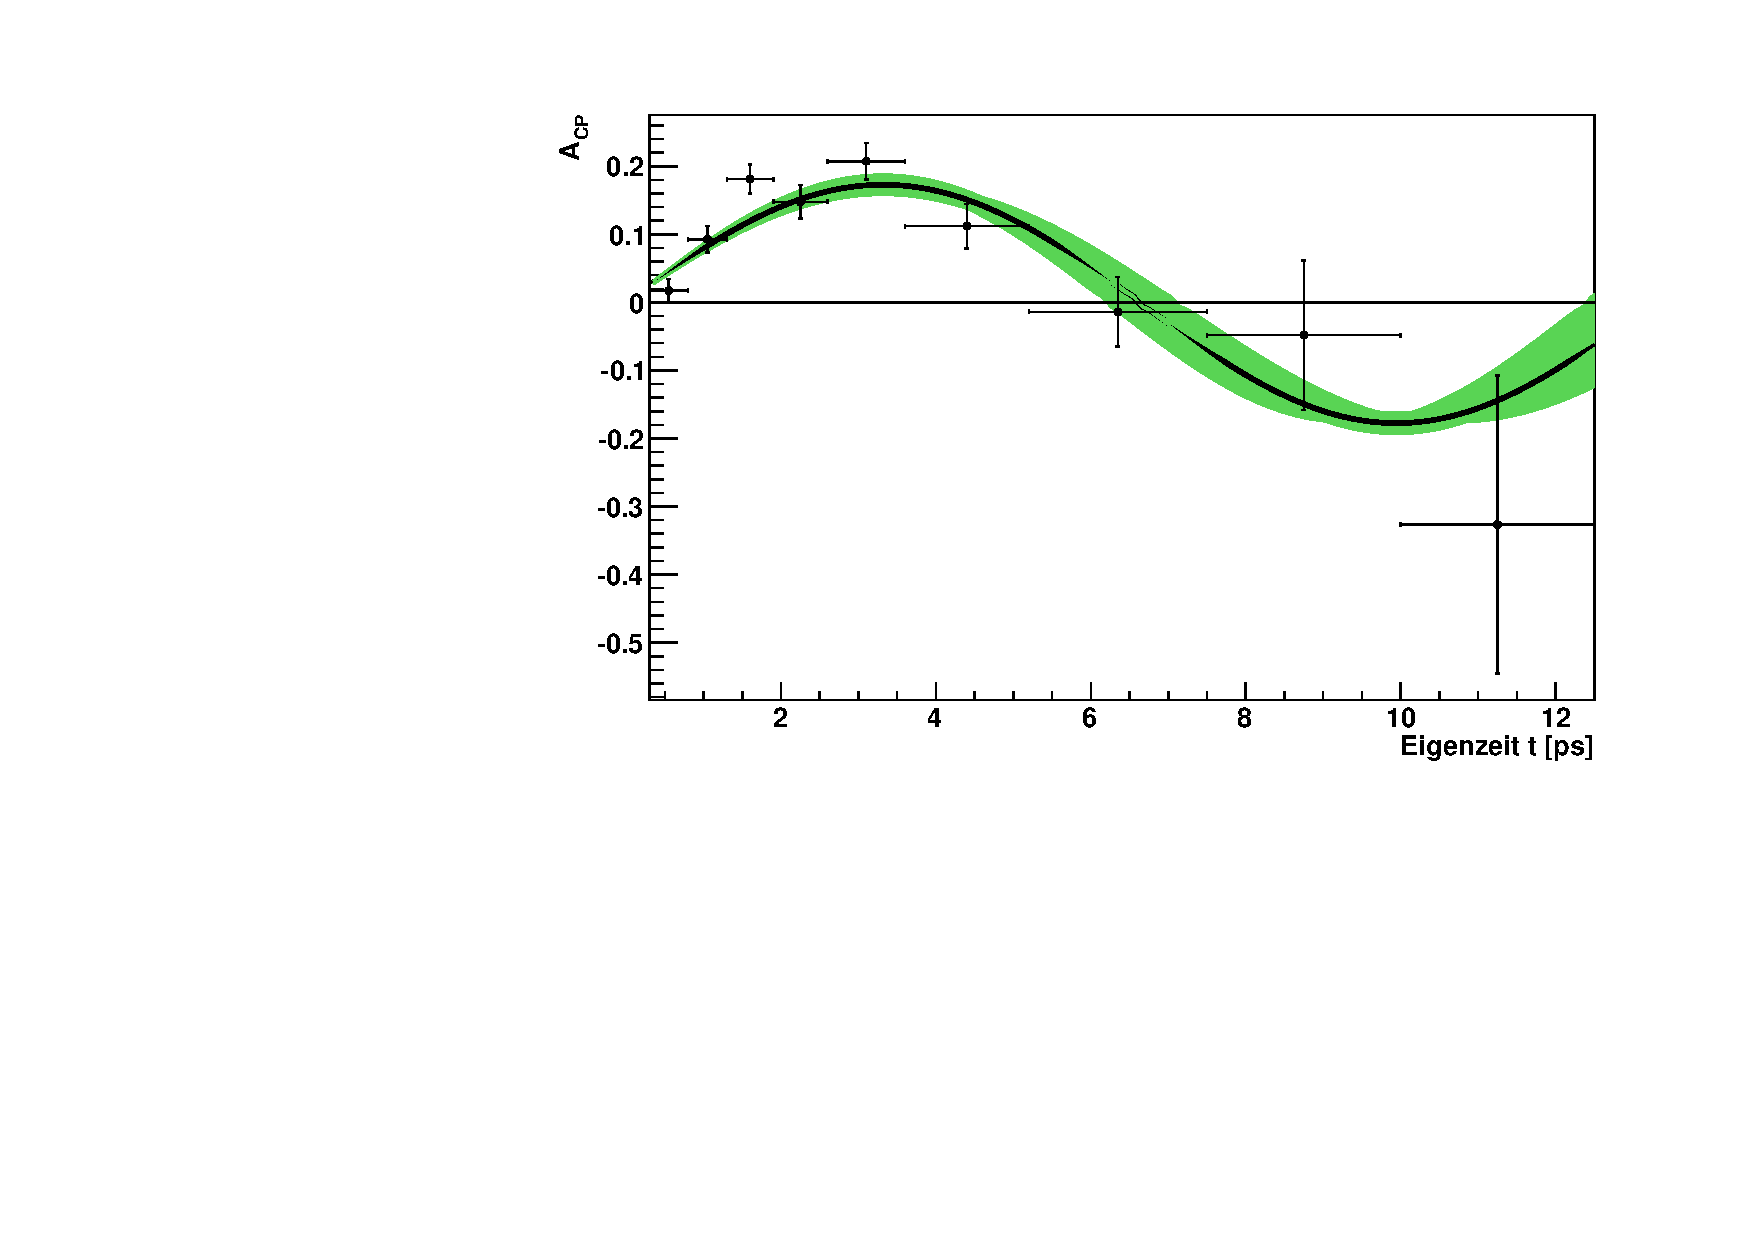
\includegraphics[width=\textwidth]{asymmetrie}
\caption{Darstellung der \CP-Asymmetrie $\mathcal{A_{CP}}$ nach Definition aus Gleichung \ref{eq:cp_asymm_def}. Für die dazugehörige Kurve wurden die aus dem Eigenzeitfit erhaltenen Parameter in Gleichung (\ref{eq:cp_asymm_meas}) eingesetzt. Das grüne Band entspricht den $1\sigma^{\text{stat.}}$ Abweichungen von $\SJPsi$ und $\Delta m_d$.}
\label{fig:asymmetrie}
\end{figure}

Abbildung \ref{fig:asymmetrie} zeigt die \CP-Asymmetrie des Signals. Die Messung von $\sin(2\beta)$ bzw. $\Delta\SJPsi$ könnte wie folgt modifiziert werden:
\begin{enumerate}
    \item Bei der Erstellung des NTupels kann die neueste Version der Analysesoftware verwendet werden, bei der die Wahrscheinlichkeit, dass es sich bei den Pionspuren um Phantome handelt, richtig kalibriert ist. Dies würde ermöglichen, bereits vor dem Fit den Datensatz etwas besser von Untergrund zu bereinigen.
    \item Als dominierende Systematik sollte der Einfluss der Kalibration der Flavour Tagging Algorithmen auf $\SJPsi$ erneut bestimmt werden, sobald die systematischen Studien des hier verwendeten Flavour Taggings abgeschlossen sind.
    \item Sobald der LHC wieder in Betrieb geht, werden mit fortlaufender Betriebsdauer mehr Daten zur Verfügung stehen, die die statistische Präzision erhöhen. Diese Analyse konnte zeigen, dass hier noch Potential besteht, da die statistische Unsicherheit etwa doppelt so groß wie die systematische ist.
\end{enumerate}



\begin{thebibliography}{---}
\bibitem{lhcb-paper} T. Brambach et al., \textit{Measurement of $\mathit{\sin(2\beta)}$ in the decay \Decaychannel\ with the 2011 LHCb data}, LHCb-ANA-2012-016.

\bibitem{pdg-average} \url{http://pdg8.lbl.gov/rpp2013v2/pdgLive/DataBlock.action?node=S042BET} (Stand: 13.08.2013).

\bibitem{cern-courier} Nico Serra, Tom Blake, \textit{Chasing new physics with electroweak penguins}, 2013 \textit{CERN Courier}, \textbf{5} 15-17.

\bibitem{roadmap} The LHCb Collaboration et al., \textit{Roadmap for selected key measurements of LHCb}, LHCb-PUB-2009-029, [\texttt{arXiv:0912.4179v3}]. 

\bibitem{lhc-info} \url{http://home.web.cern.ch/about/accelerators/large-hadron-collider} (Stand: 01.08.2013).

\bibitem{lhcb-info} \url{http://www.weltmaschine.de/experimente/lhcb/} (Stand: 01.08.2013).

\bibitem{detektorakzeptanz} Johan Luisier, \textit{Measurement of B-meson lifetime ratios with the LHCb detector}, 2011. Dissertation erreichbar unter \url{http://lphe.epfl.ch/publications/theses/these.jl.pdf} (Stand: 15.08.2013).

\bibitem{thesis_linn} Christian Linn, \textit{Measurement of the CP-violating phase $\Phi_{\text{s}}$ using $B_s^0 \rightarrow J/\Psi\Phi$ and $B_s^0 \rightarrow J/\Psi\pi^+\pi^-$ decays with the LHCb experiment}, 2013. Dissertation erreichbar unter \url{http://www.physi.uni-heidelberg.de//Publications/linn_thesis.pdf} (Stand: 13.08.2013).

\bibitem{detector} The LHCb Collaboration et al., \textit{The LHCb Detector at the LHC}, 2008 \textit{JINST}, \textbf{3} S08005.

\bibitem{wiki_standard} \url{http://commons.wikimedia.org/wiki/File:Standard_Model_of_Elementary_Particles-de.svg} (Stand: 07.07.2013).

\bibitem{higgs} CERN, Pressemitteilung, 2013, \url{http://press.web.cern.ch/press-releases/2013/03/new-results-indicate-particle-discovered-cern-higgs-boson} (Stand: 13.08.2013).

\bibitem{wu-experiment} C.S. Wu, \textit{Experimental Test of Parity Conservation in Beta Decay}, 1957 Phys. Rev., \textbf{105} 1413-1415.

\bibitem{kleinknecht}  Konrad Kleinknecht, \textit{Uncovering \CP\ Violation}, \textit{Experimental Clarification in the Neutral K Meson and B Meson Systems}, Springer, Heidelberg, 2003.

\bibitem{dreieck} \url{http://inspirehep.net/record/1085541/files/figs_CKM_triangle.png} (Stand: 03.08.2013).

\bibitem{nir} Yosef Nir, \textit{The CKM Matrix and New Physics}, 2003 \textit{Nucl. Phys. B (Proc. Suppl.)}, \textbf{117} 111-116.

\bibitem{noguchi} S. Noguchi, \textit{CP violation in B Meson Decays}, 2003 \textit{Nucl. Phys. A}, \textbf{721} 151c-160c.

\bibitem{trigger} \url{http://lhcb-trig.web.cern.ch/lhcb-trig/} (Stand: 13.08.2013).

\bibitem{sfit} Yuehong Xie, \textit{sFit: a method for background subtraction in maximum likelihood fit}, 2009, [\texttt{arXiv:0905.0724v1}].

\bibitem{splot} M. Pivk, F.R. Le Diberder, \SPlot\textit{: a statistical tool to unfold data distributions}, 2005, [\texttt{arXiv:physics/0402083v3}].

\bibitem{tagging} Stefania Vecchi, \textit{OS combination for Reco14}, 2013, LHCb Flavour Tagging Meeting 20.06.2013.

\bibitem{2010-analyse} T. Brambach et al., \textit{Measurement of CP violation in the time-dependent analysis of \Decaychannel\ decays with the 2010 data}, LHCb-ANA-2011-004.

\bibitem{crystal_ball} The CMS Collaboration, \textit{Suppression of non-prompt $J/\Psi$, prompt $J/\Psi$, and $\Upsilon$(1S)
in PbPb collisions at $\sqrt{s_{NN}} = 2.76 \tera\electronvolt$}, 2013, [\texttt{arXiv:1201.5069v2}].

\bibitem{pdg-tau} \url{http://pdglive.lbl.gov/popupblockdata.brl?nodein=S042T&inscript=Y&fsizein=1&clumpin0=} (Stand: 02.07.2013).

\end{thebibliography}

% Selbstständigkeitserklärung
\chapter*{Erklärung}

Ich versichere, dass ich diese Arbeit selbstständig verfasst und keine anderen als die angegebenen Quellen und Hilfsmittel benutzt habe. \\
\vspace{0.2cm}
\begin{flushleft}
Heidelberg, den 19.08.2013,\\
\vspace{2cm}
%Unterschrift
Patrick Fahner
\end{flushleft}



\end{document}


